\documentclass[../main.tex]{subfiles}

\begin{document}

%%%%%%%%%%%%%%%%%%%%%%%%%%%%%%%%%%%
%
%	Read Depth SnapShots
%
%%%%%%%%%%%%%%%%%%%%%%%%%%%%%%%%%%%

In order to attempt to gain a understanding of the read depth landscape that exists in the fifteen strains "snapshots" of the regions where it had been identified by Hao that there were notably high read depths. These snapshots consist of the region identified as having high read depth as well as the regions $\pm$500 points from the high read depth bounds. Below are a few examples of the regions with high read depth for one of the strains, only a few of the snapshots could be displayed because Hao identified upwards of 4000 regions with high read depth for each strain.

\begin{table}[H]
	\begin{center}
	\captionof{table}{Total number of locations of high read depths identified by Hao} \label{tab:sitesctjnum}
	\vspace{0.5cm}
	\scalebox{.5}{
	\begin{tabular}{ |c|c| } 
		\hline
		Strain & Num Significant Read depths\\
		\hline
		Ar73 & 2248\\
		\hline	
		Ar109 & 4392\\
		\hline
		Ar119 & 3867\\
		\hline
		Ar142 & 2796\\
		\hline
		Ar159 & 3343\\
		\hline
		Ar170 & 2044\\
		\hline
		Ar174 & 1964\\
		\hline
		Ar175 & 2245\\
		\hline
		Ar176 & 2278\\
		\hline
		Ar179 & 2172\\
		\hline
		Ar188 & 3242\\
		\hline
		Ar194 & 2397\\
		\hline
		Ar196 & 2314\\
		\hline
		Ar201 & 2233\\
		\hline
		Ar213 & 2000\\
		\hline
	\end{tabular}
	}
	\end{center}
\end{table}
\begin{figure}[H]
	\begin{centering}
		\resizebox{40mm}{40mm}{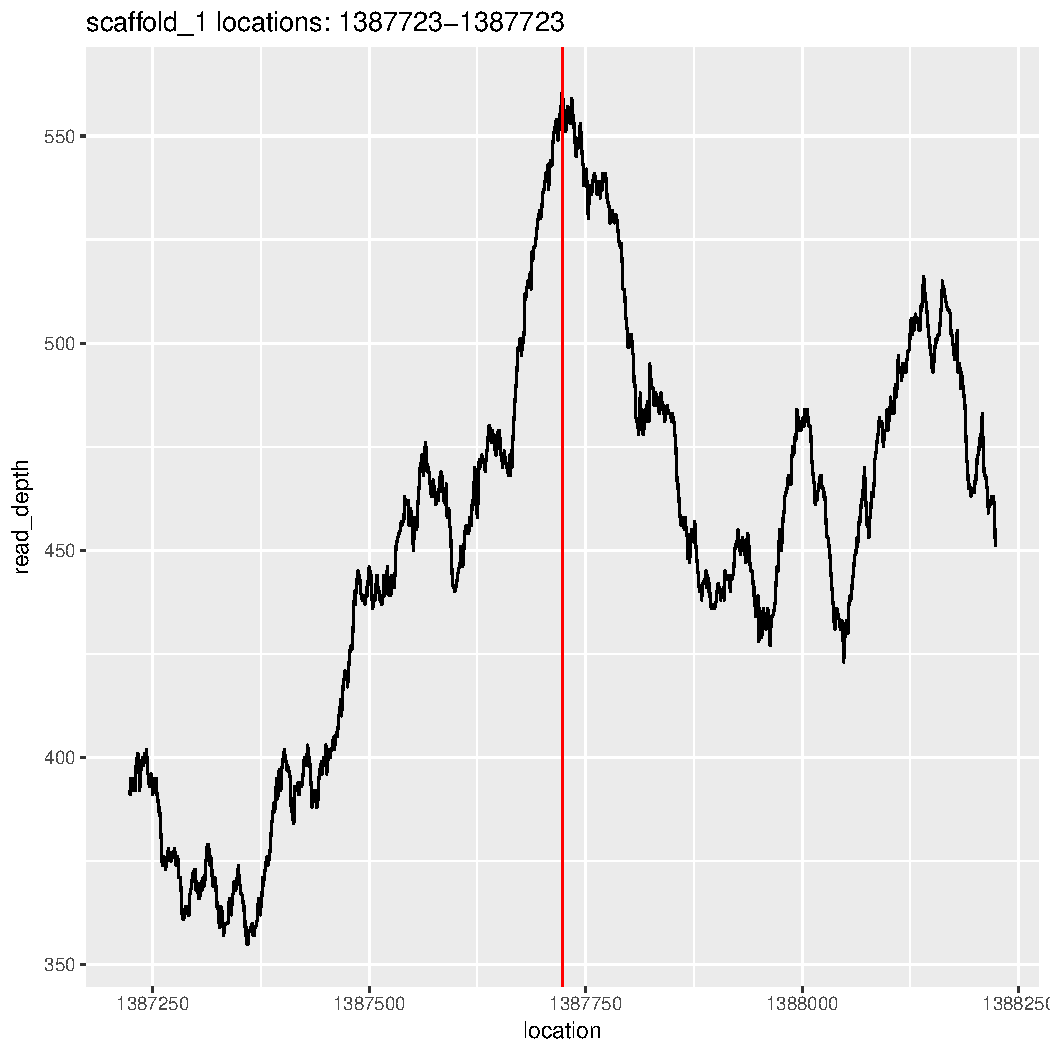
\includegraphics[angle=0,width=1.0\linewidth]{Figures/read_depth_snapsots/1_Ar109_read_depth.pdf}}
		\resizebox{40mm}{40mm}{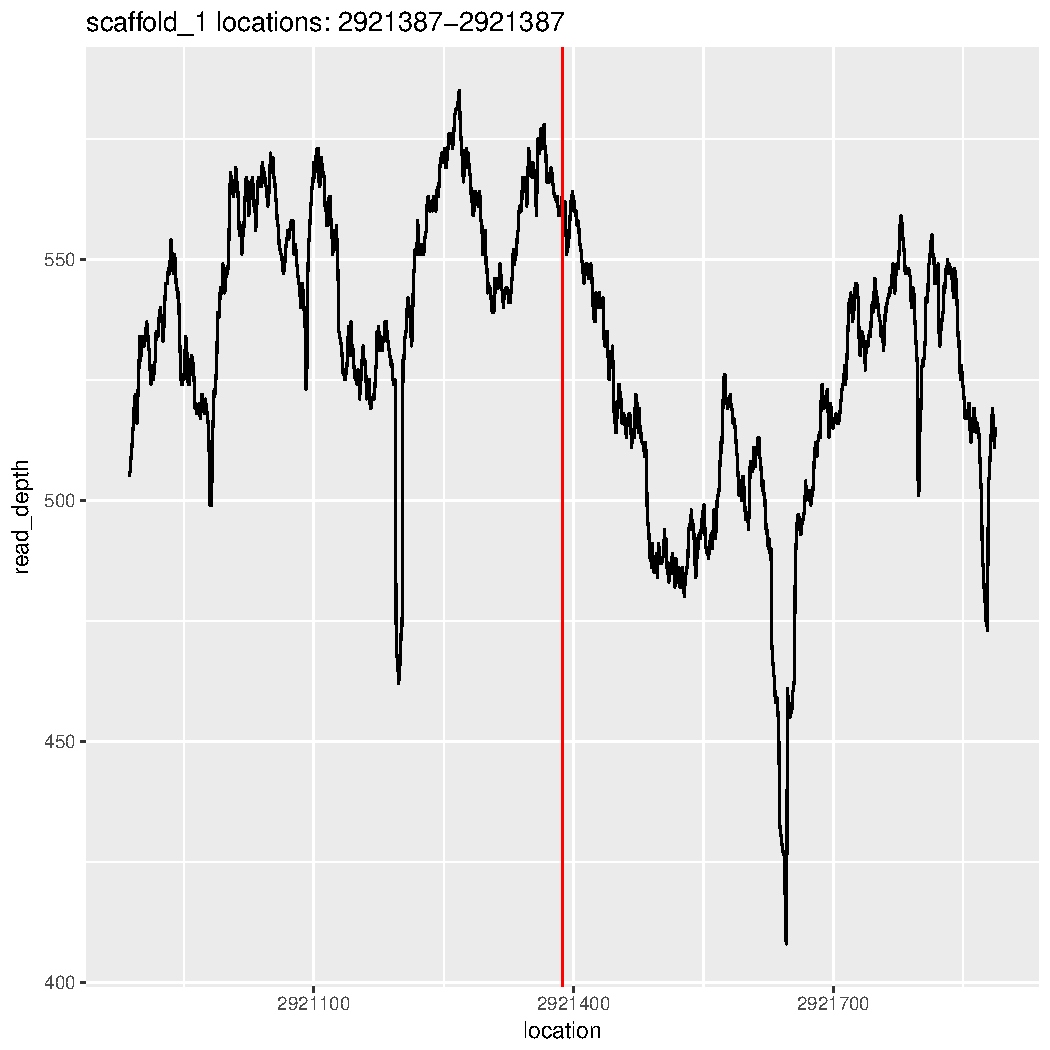
\includegraphics[angle=0,width=1.0\linewidth]{Figures/read_depth_snapsots/100_Ar109_read_depth.pdf}}
		\resizebox{40mm}{40mm}{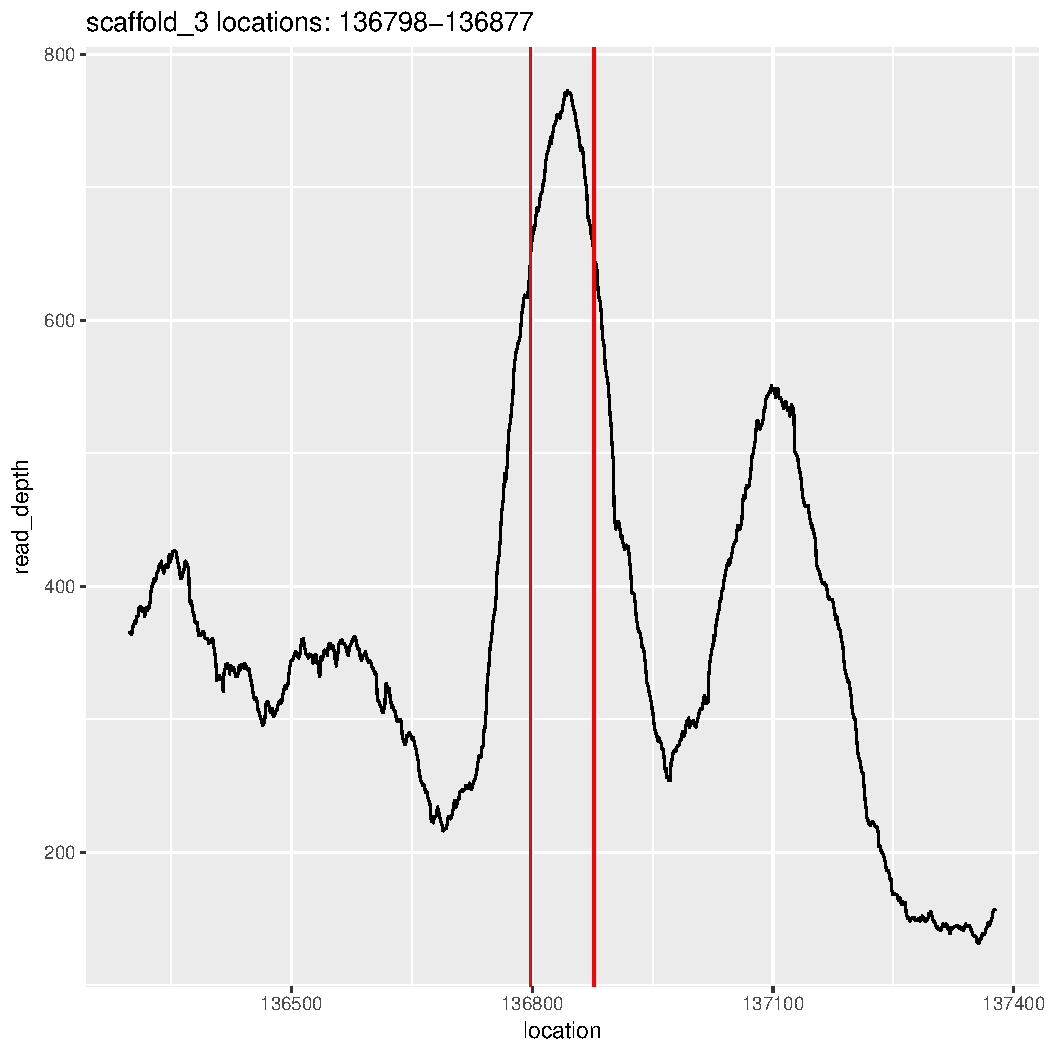
\includegraphics[angle=0,width=1.0\linewidth]{Figures/read_depth_snapsots/200_Ar109_read_depth.pdf}}
		\resizebox{40mm}{40mm}{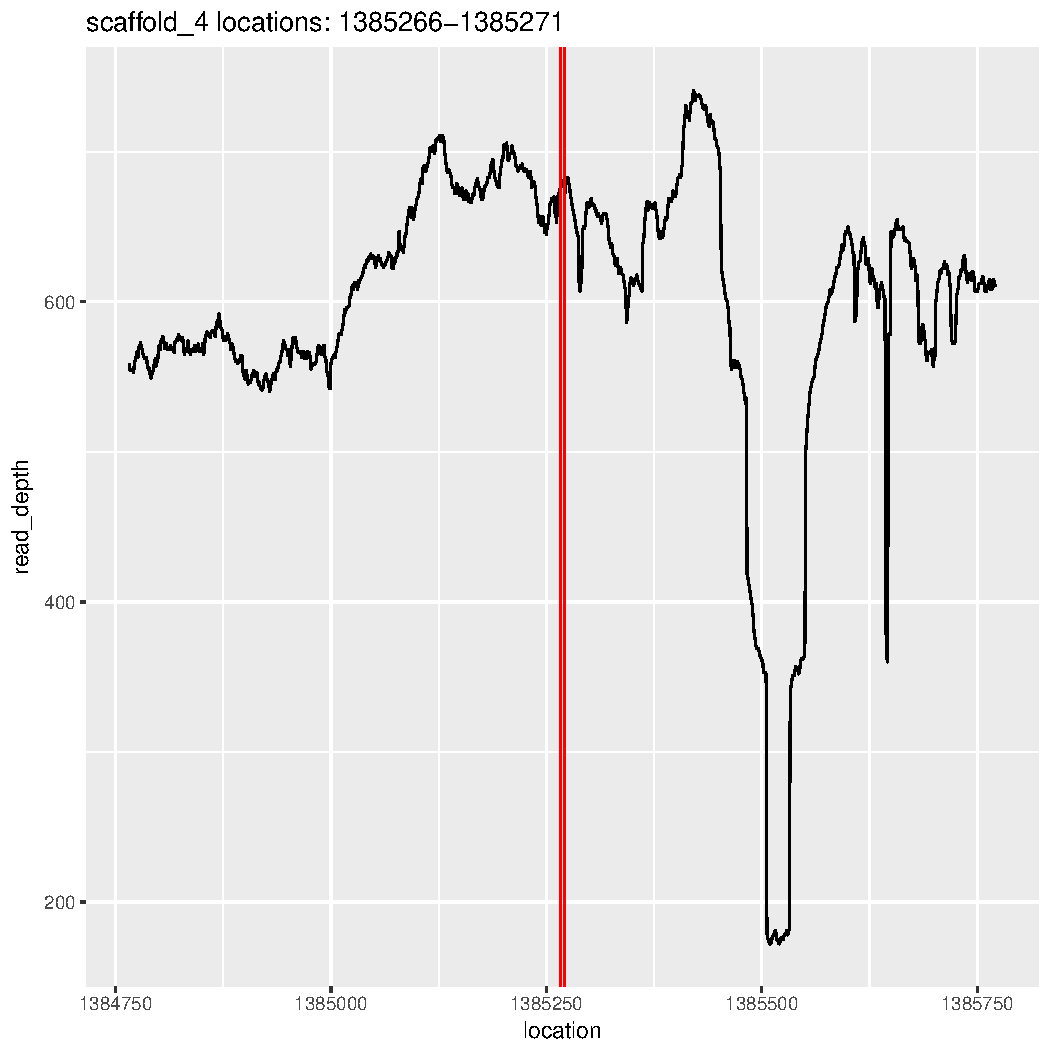
\includegraphics[angle=0,width=1.0\linewidth]{Figures/read_depth_snapsots/300_Ar109_read_depth.pdf}}
		\resizebox{40mm}{40mm}{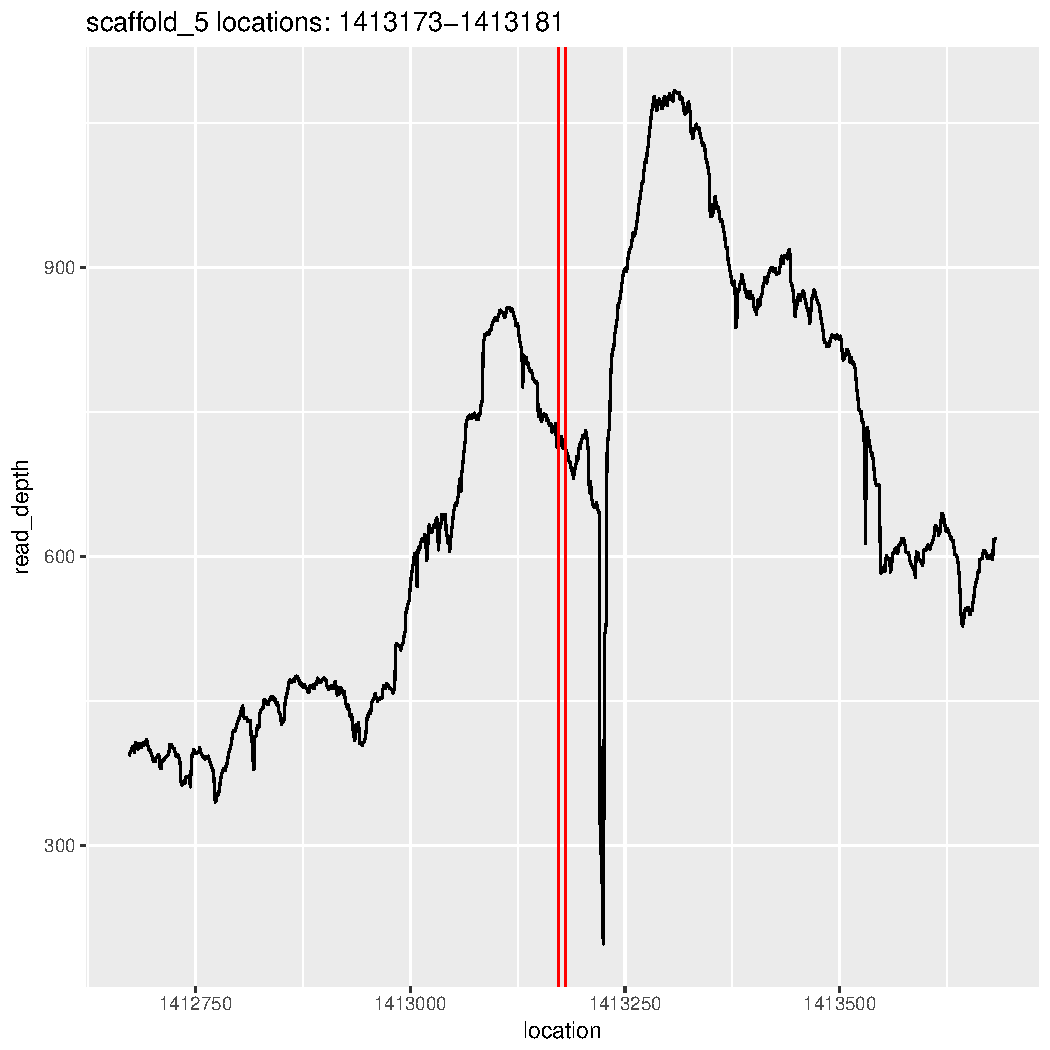
\includegraphics[angle=0,width=1.0\linewidth]{Figures/read_depth_snapsots/400_Ar109_read_depth.pdf}}
		\resizebox{40mm}{40mm}{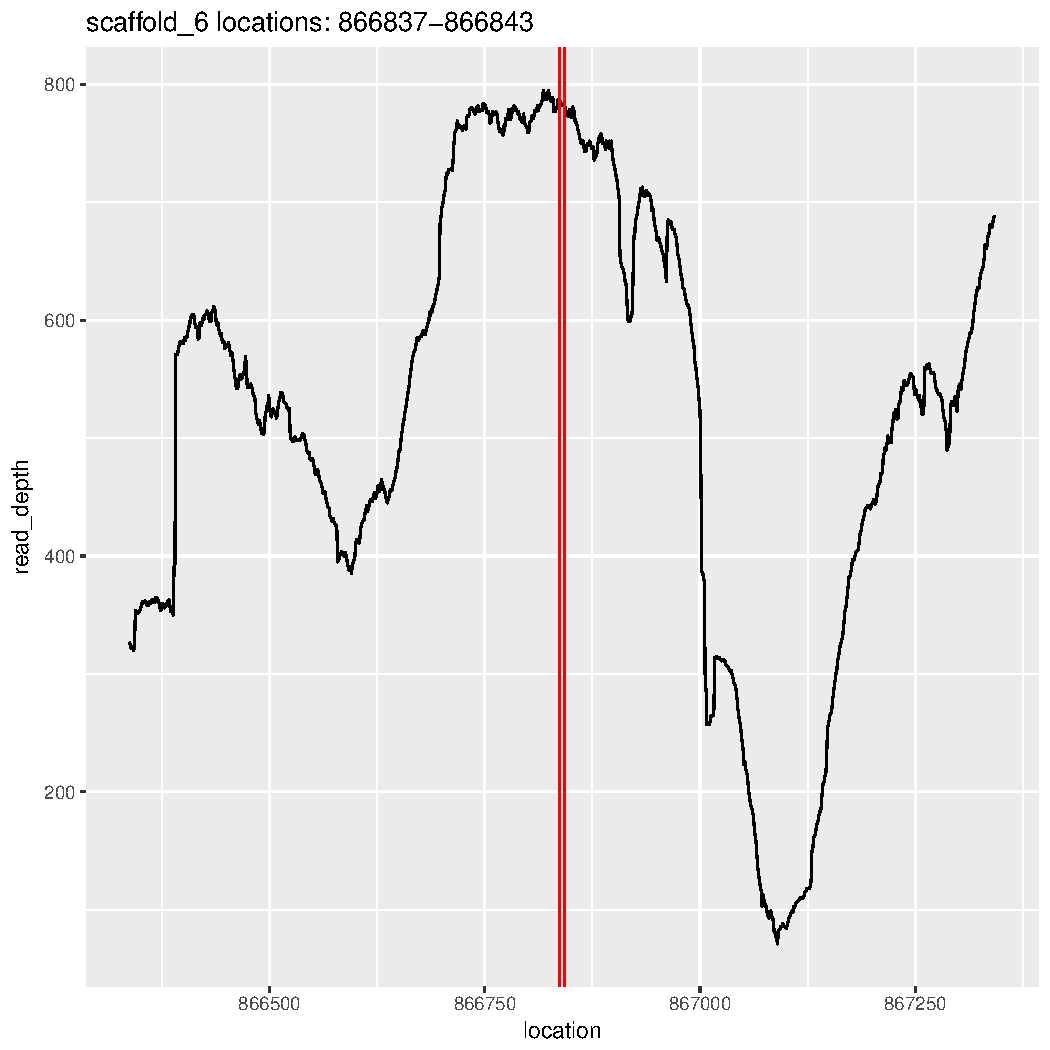
\includegraphics[angle=0,width=1.0\linewidth]{Figures/read_depth_snapsots/500_Ar109_read_depth.pdf}}
		\resizebox{40mm}{40mm}{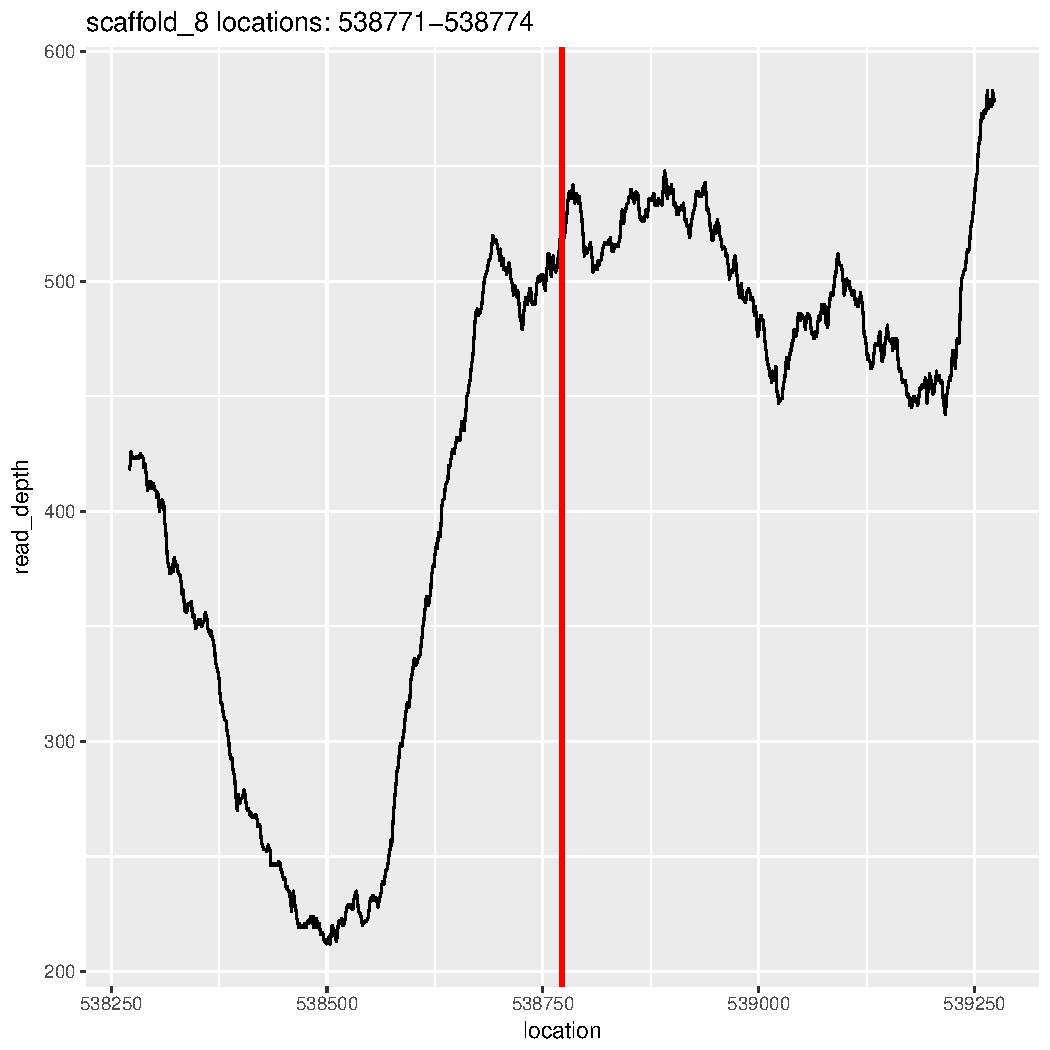
\includegraphics[angle=0,width=1.0\linewidth]{Figures/read_depth_snapsots/600_Ar109_read_depth.pdf}}
		\resizebox{40mm}{40mm}{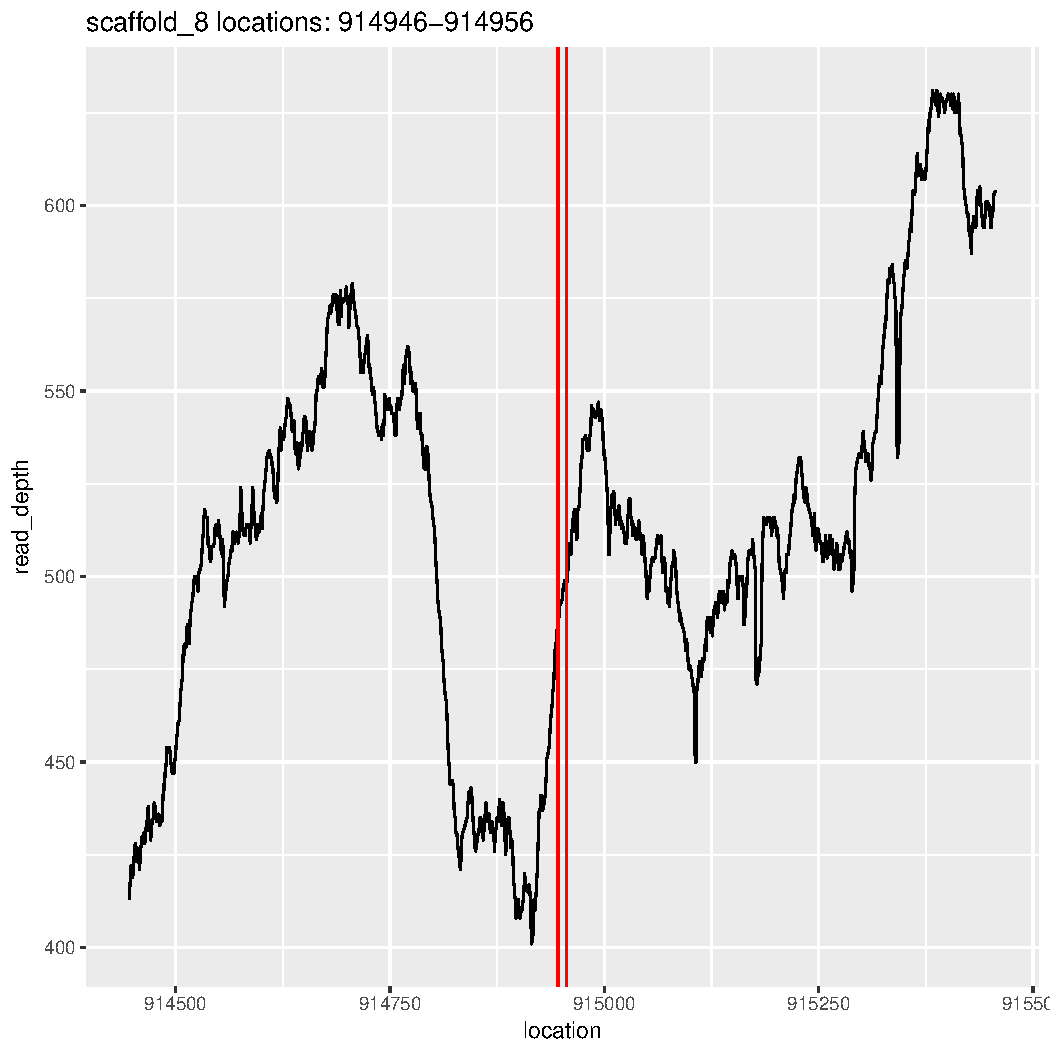
\includegraphics[angle=0,width=1.0\linewidth]{Figures/read_depth_snapsots/700_Ar109_read_depth.pdf}}
		\resizebox{40mm}{40mm}{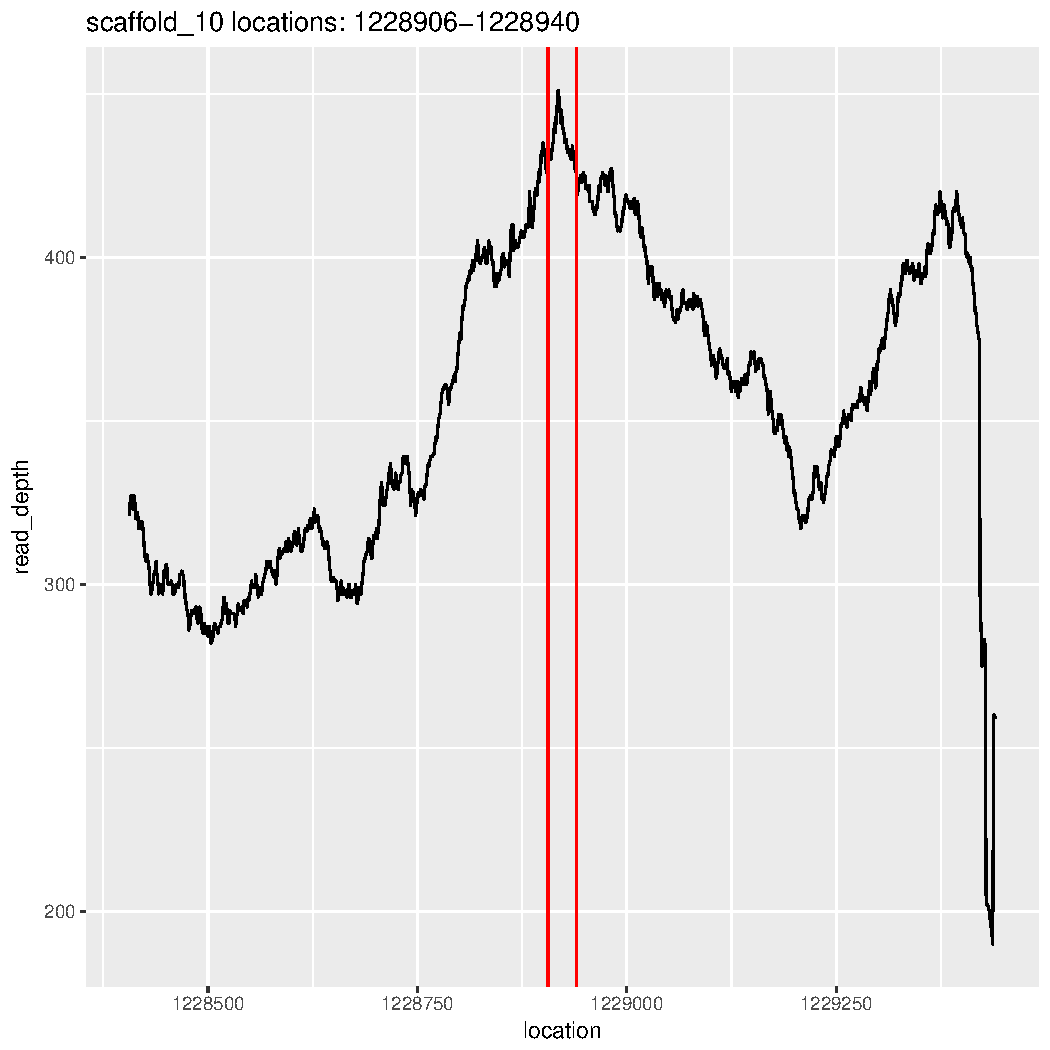
\includegraphics[angle=0,width=1.0\linewidth]{Figures/read_depth_snapsots/800_Ar109_read_depth.pdf}}
		\resizebox{40mm}{40mm}{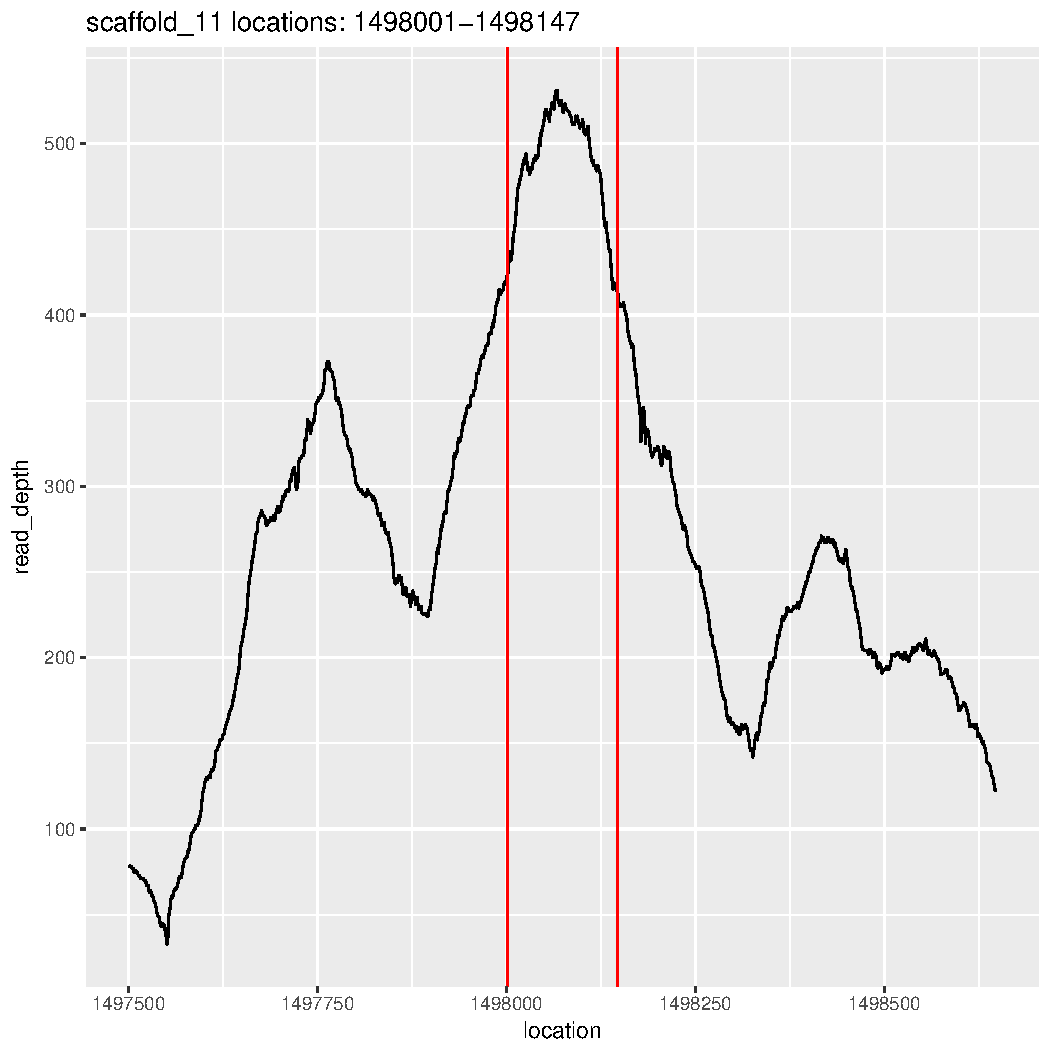
\includegraphics[angle=0,width=1.0\linewidth]{Figures/read_depth_snapsots/900_Ar109_read_depth.pdf}}
		\resizebox{40mm}{40mm}{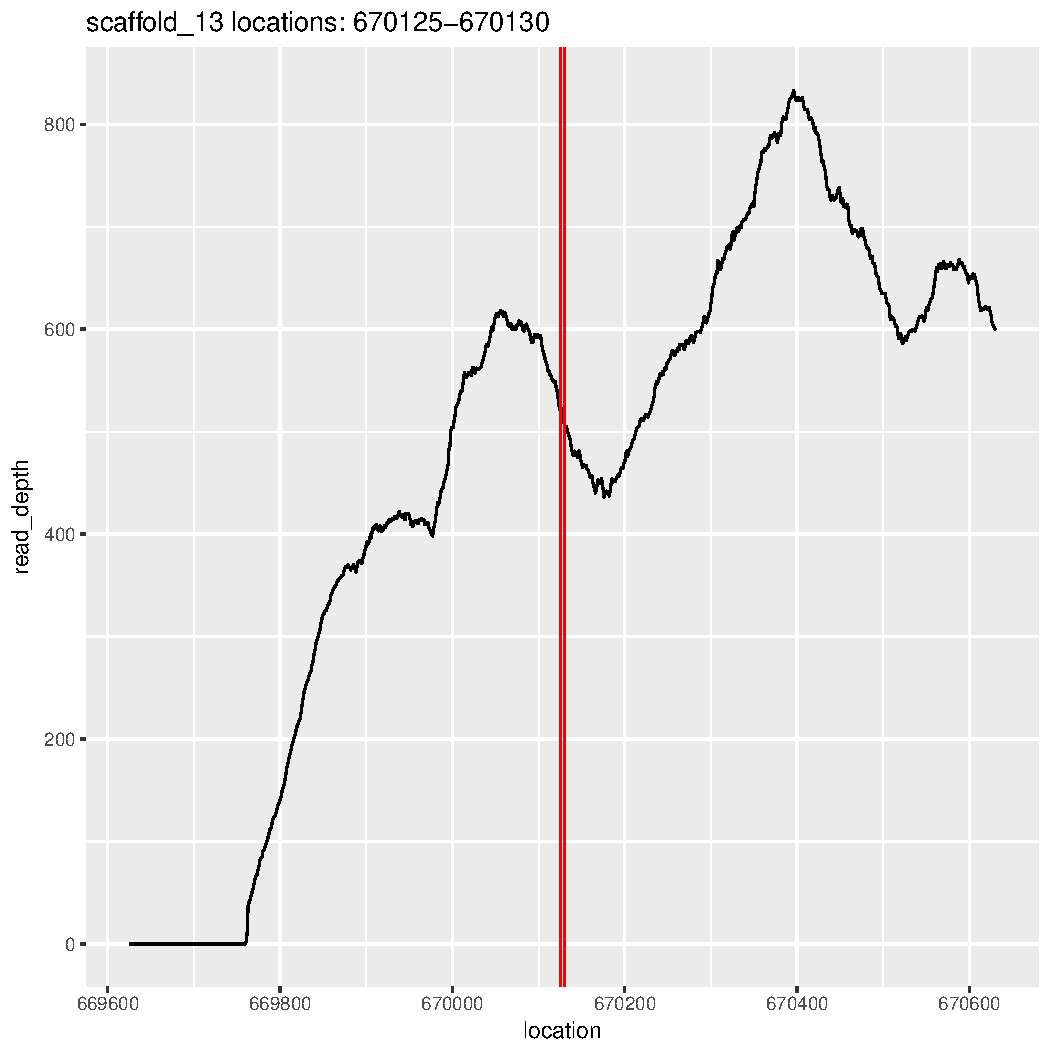
\includegraphics[angle=0,width=1.0\linewidth]{Figures/read_depth_snapsots/1000_Ar109_read_depth.pdf}}
		\resizebox{40mm}{40mm}{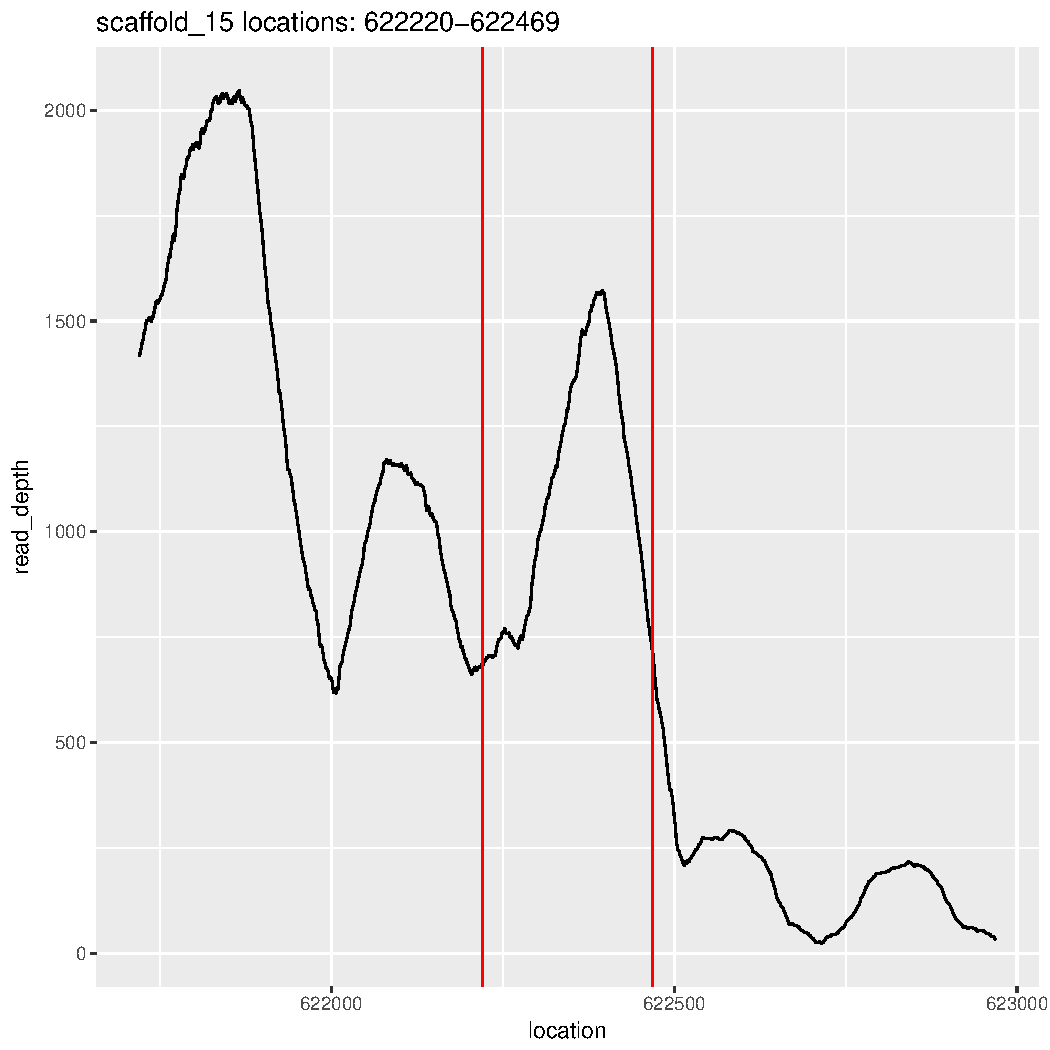
\includegraphics[angle=0,width=1.0\linewidth]{Figures/read_depth_snapsots/1100_Ar109_read_depth.pdf}}
		\resizebox{40mm}{40mm}{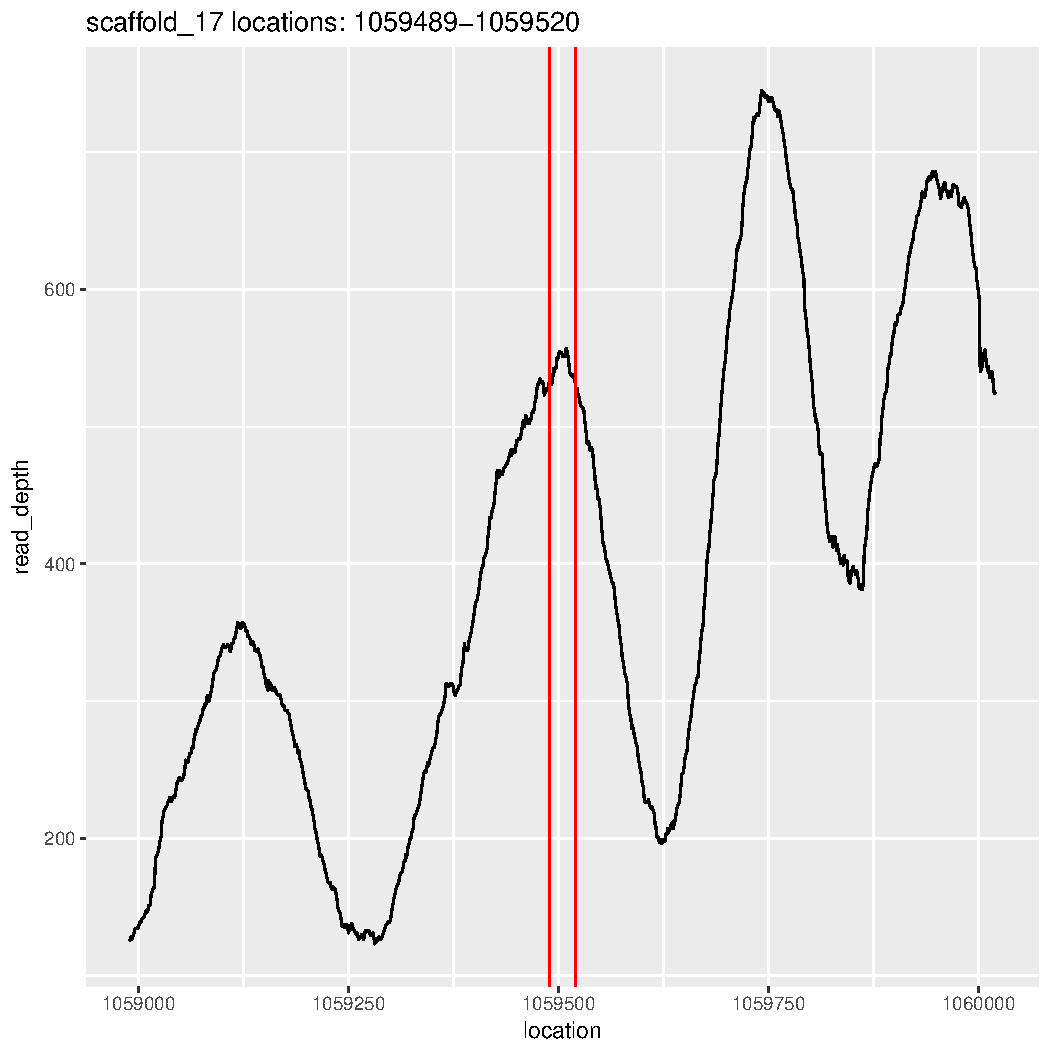
\includegraphics[angle=0,width=1.0\linewidth]{Figures/read_depth_snapsots/1200_Ar109_read_depth.pdf}}
		\resizebox{40mm}{40mm}{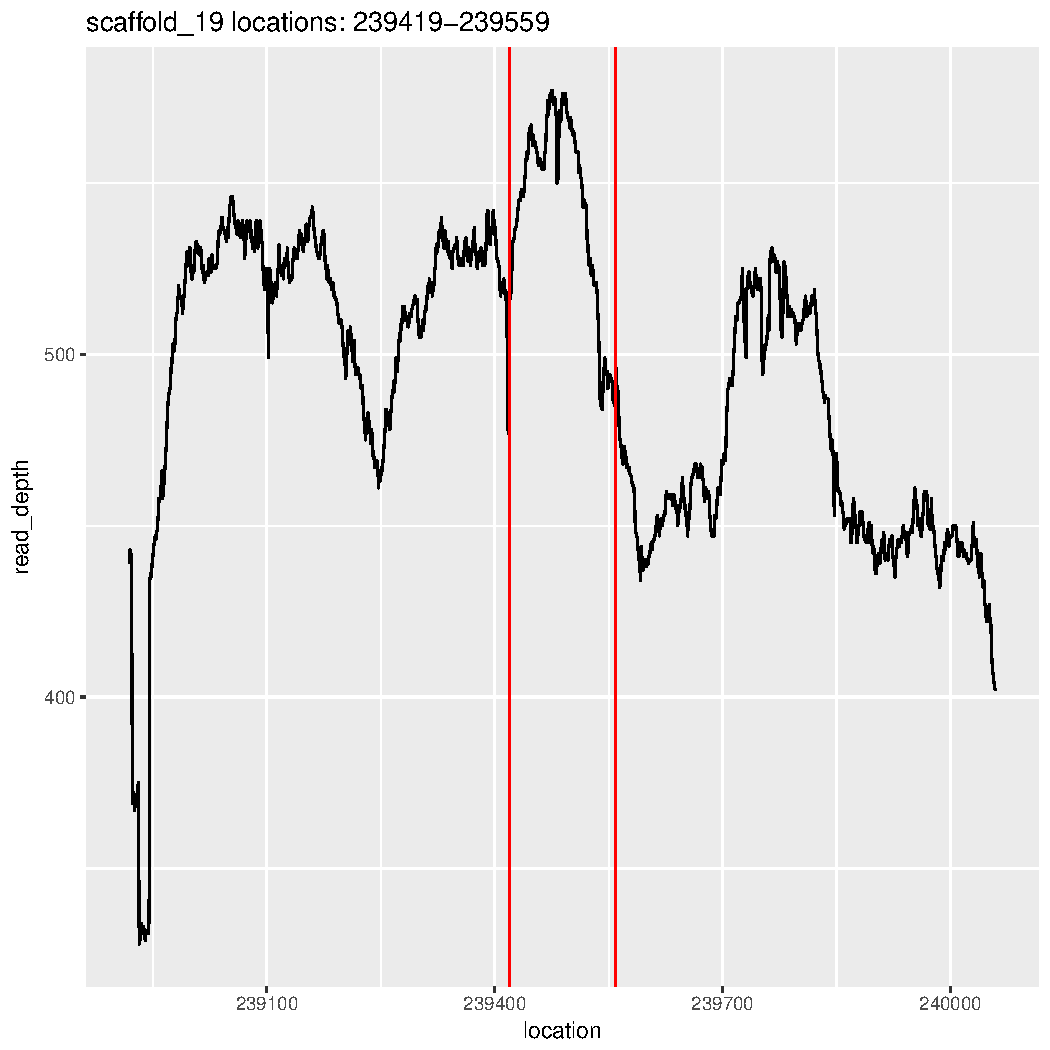
\includegraphics[angle=0,width=1.0\linewidth]{Figures/read_depth_snapsots/1300_Ar109_read_depth.pdf}}
		\resizebox{40mm}{40mm}{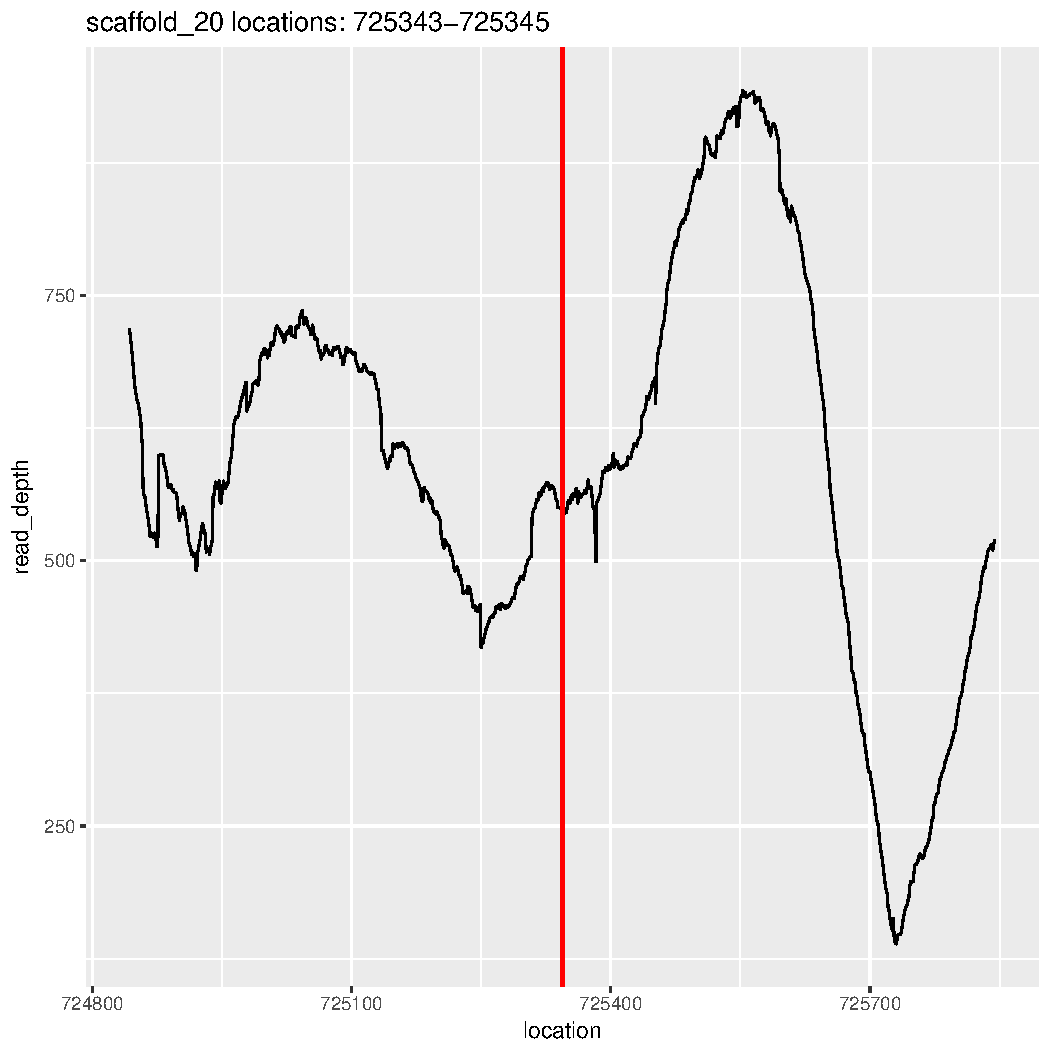
\includegraphics[angle=0,width=1.0\linewidth]{Figures/read_depth_snapsots/1400_Ar109_read_depth.pdf}}
		\resizebox{40mm}{40mm}{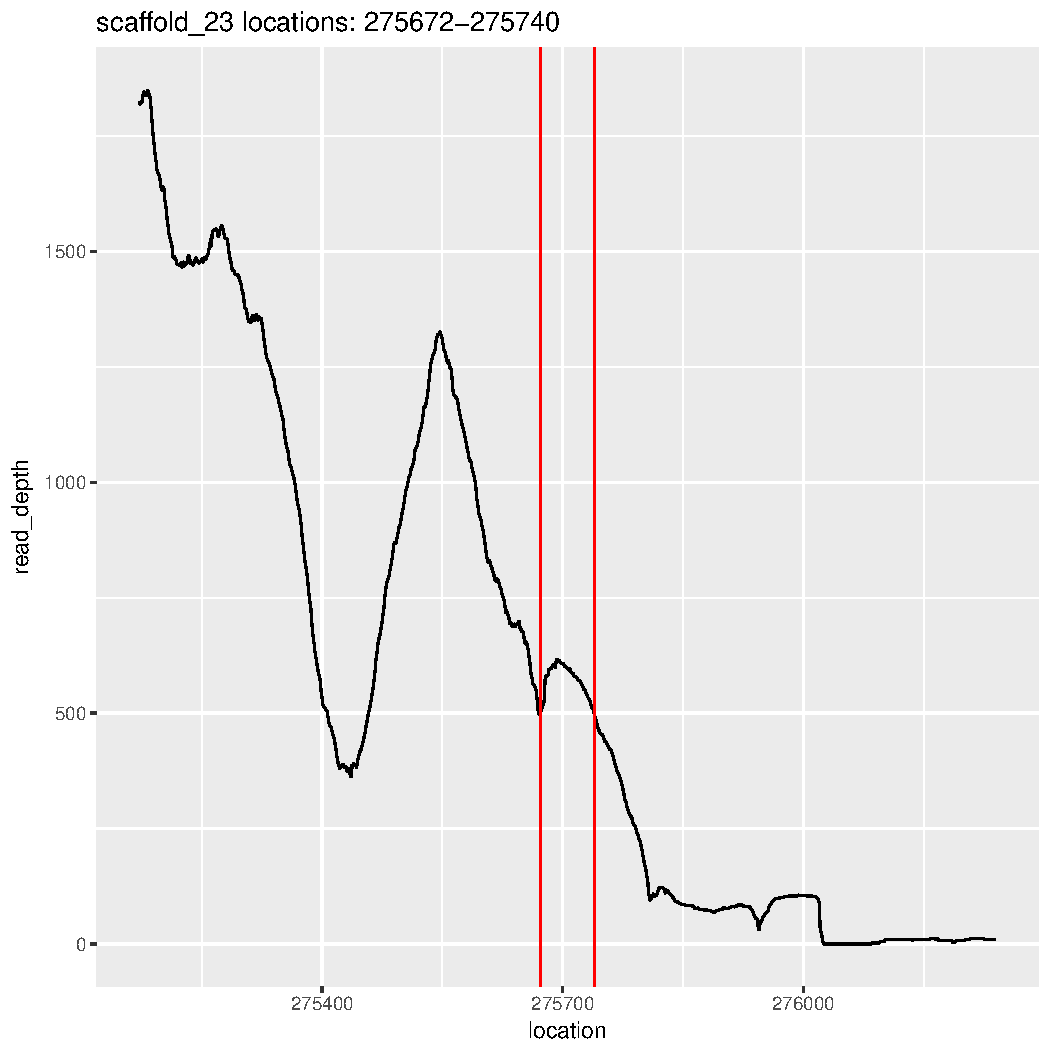
\includegraphics[angle=0,width=1.0\linewidth]{Figures/read_depth_snapsots/1500_Ar109_read_depth.pdf}}
		\resizebox{40mm}{40mm}{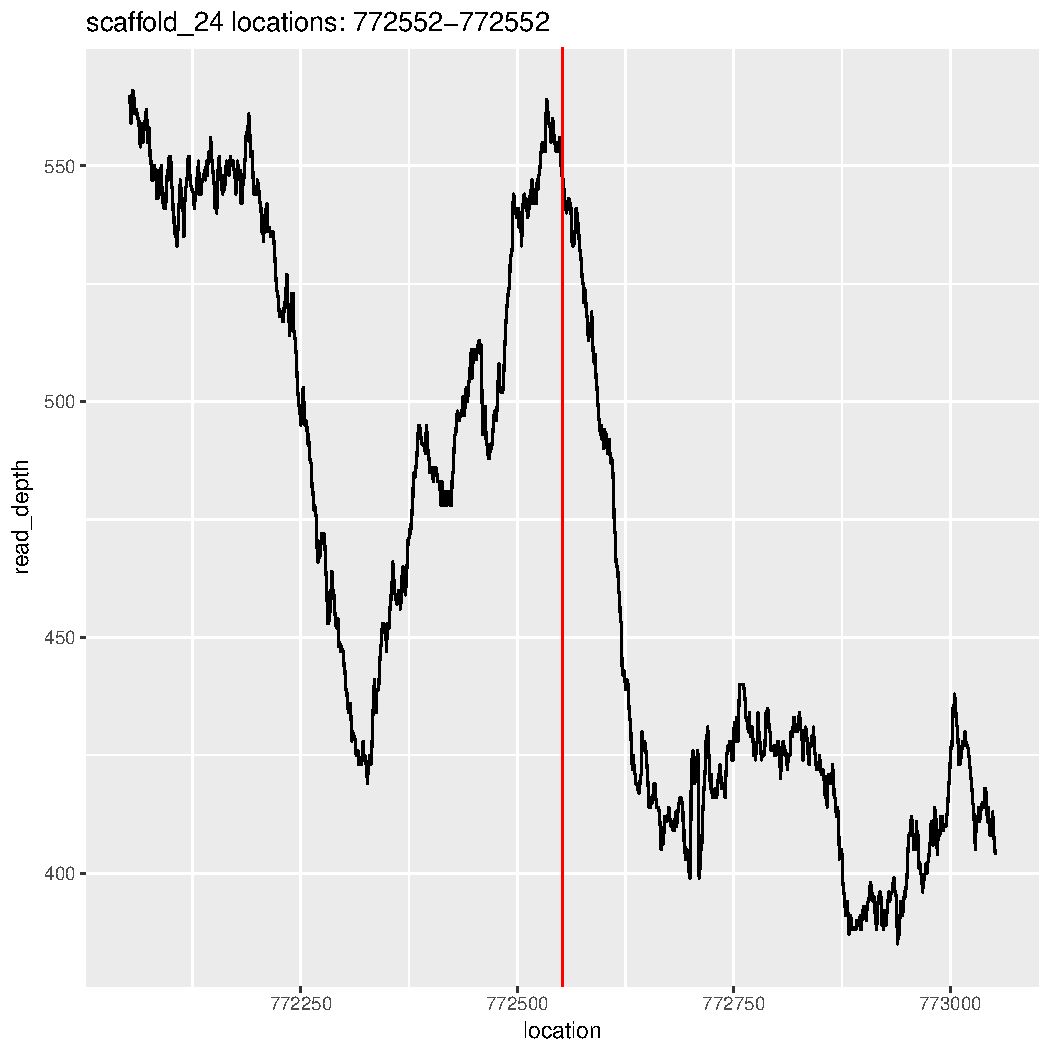
\includegraphics[angle=0,width=1.0\linewidth]{Figures/read_depth_snapsots/1600_Ar109_read_depth.pdf}}
		\resizebox{40mm}{40mm}{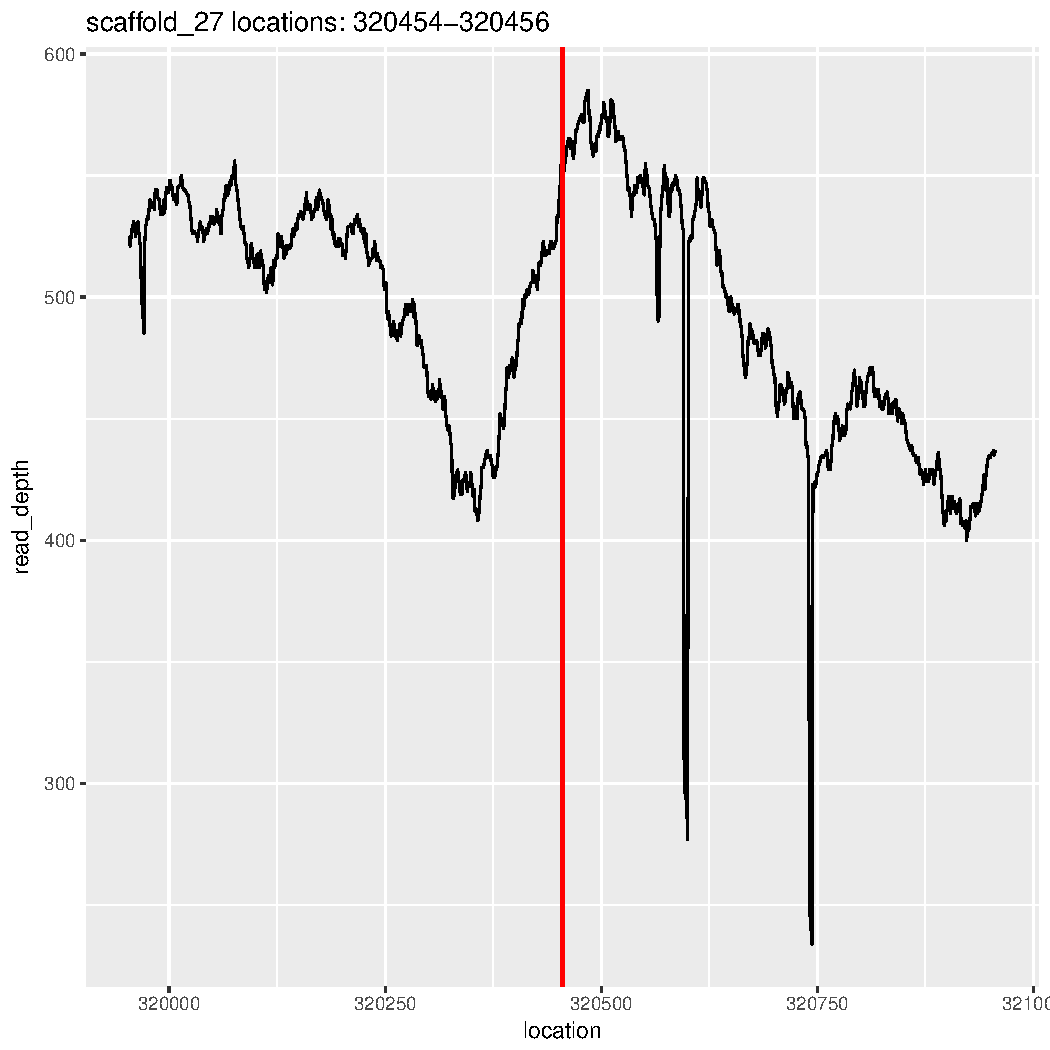
\includegraphics[angle=0,width=1.0\linewidth]{Figures/read_depth_snapsots/1700_Ar109_read_depth.pdf}}
		\resizebox{40mm}{40mm}{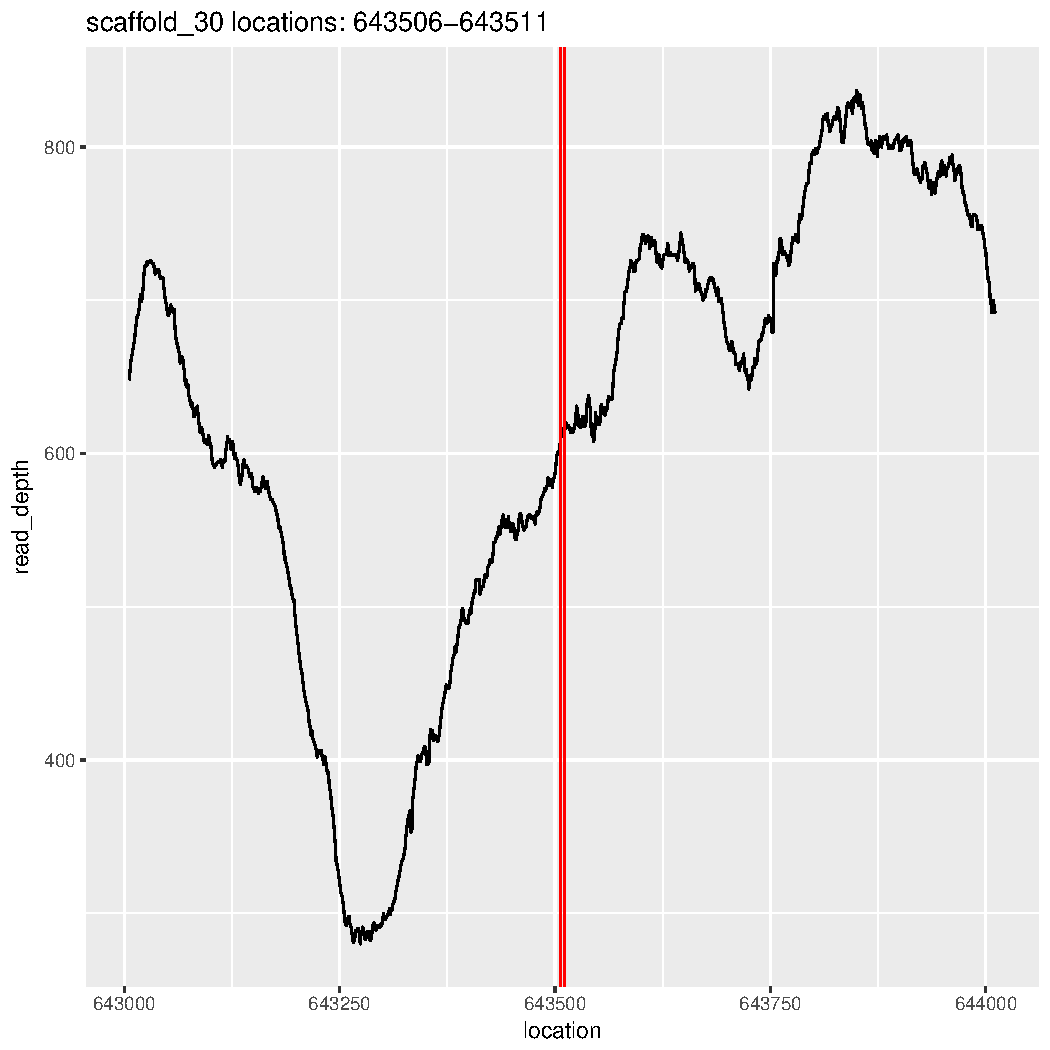
\includegraphics[angle=0,width=1.0\linewidth]{Figures/read_depth_snapsots/1800_Ar109_read_depth.pdf}}
		\resizebox{40mm}{40mm}{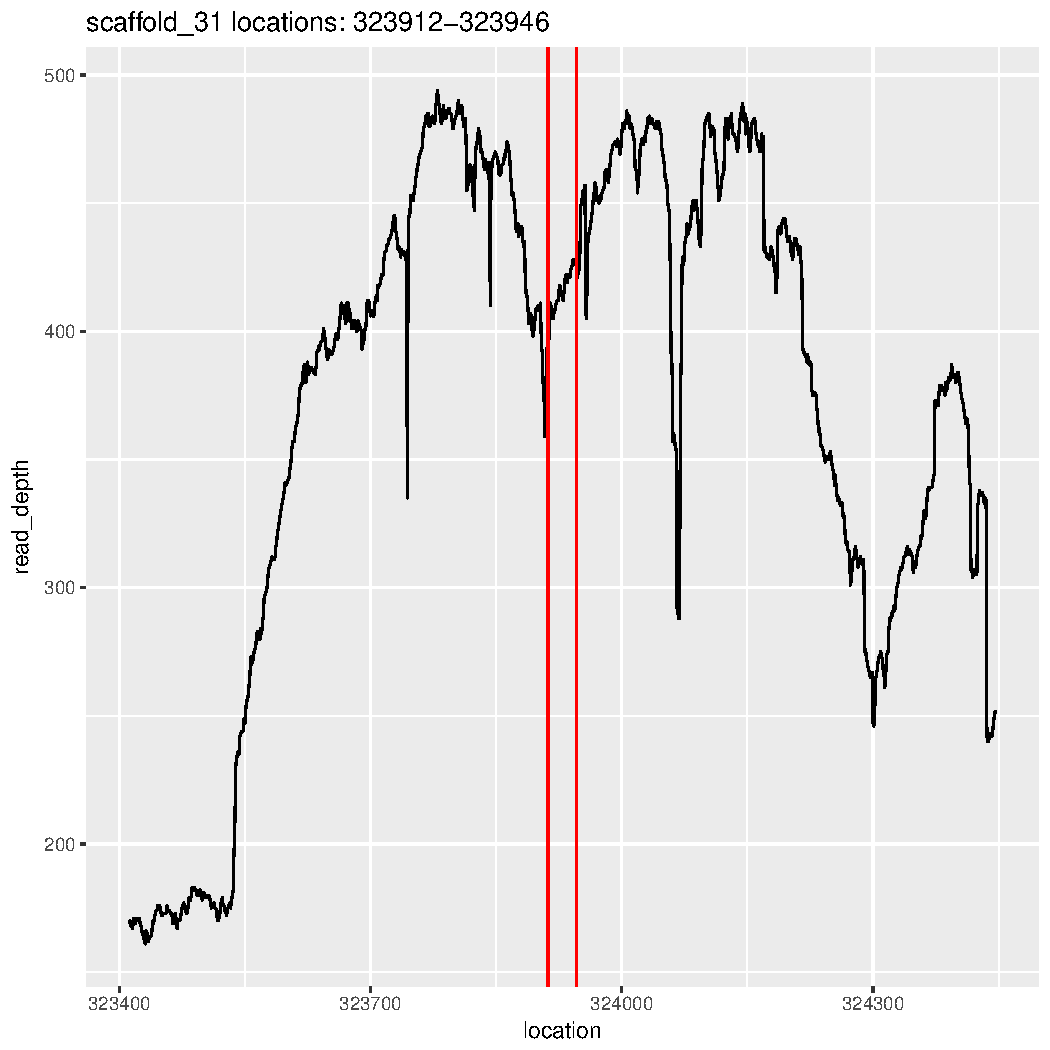
\includegraphics[angle=0,width=1.0\linewidth]{Figures/read_depth_snapsots/1900_Ar109_read_depth.pdf}}
		\begin{singlespace}
			\vspace{-0.5cm}
			\caption[Average Read Depth Snapshots]{Average Read Depth Snapshots. Graphs are of locations 1, and every 100 starting at 100 until 1900.}\label{avg_rd_snpsht_1}
		\end{singlespace}
	\end{centering}
\end{figure}
\begin{figure}[H]
	\begin{centering}
		\resizebox{40mm}{40mm}{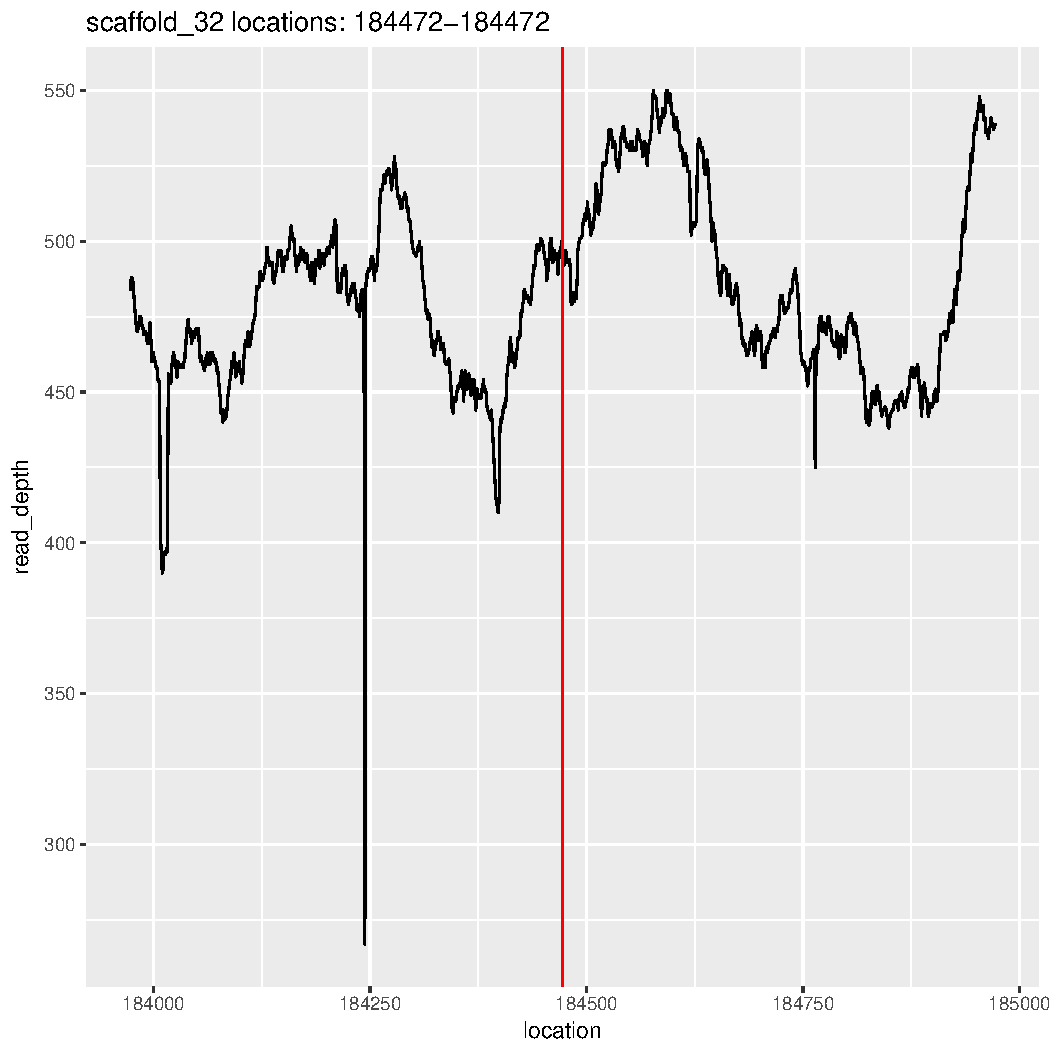
\includegraphics[angle=0,width=1.0\linewidth]{Figures/read_depth_snapsots/2000_Ar109_read_depth.pdf}}
		\resizebox{40mm}{40mm}{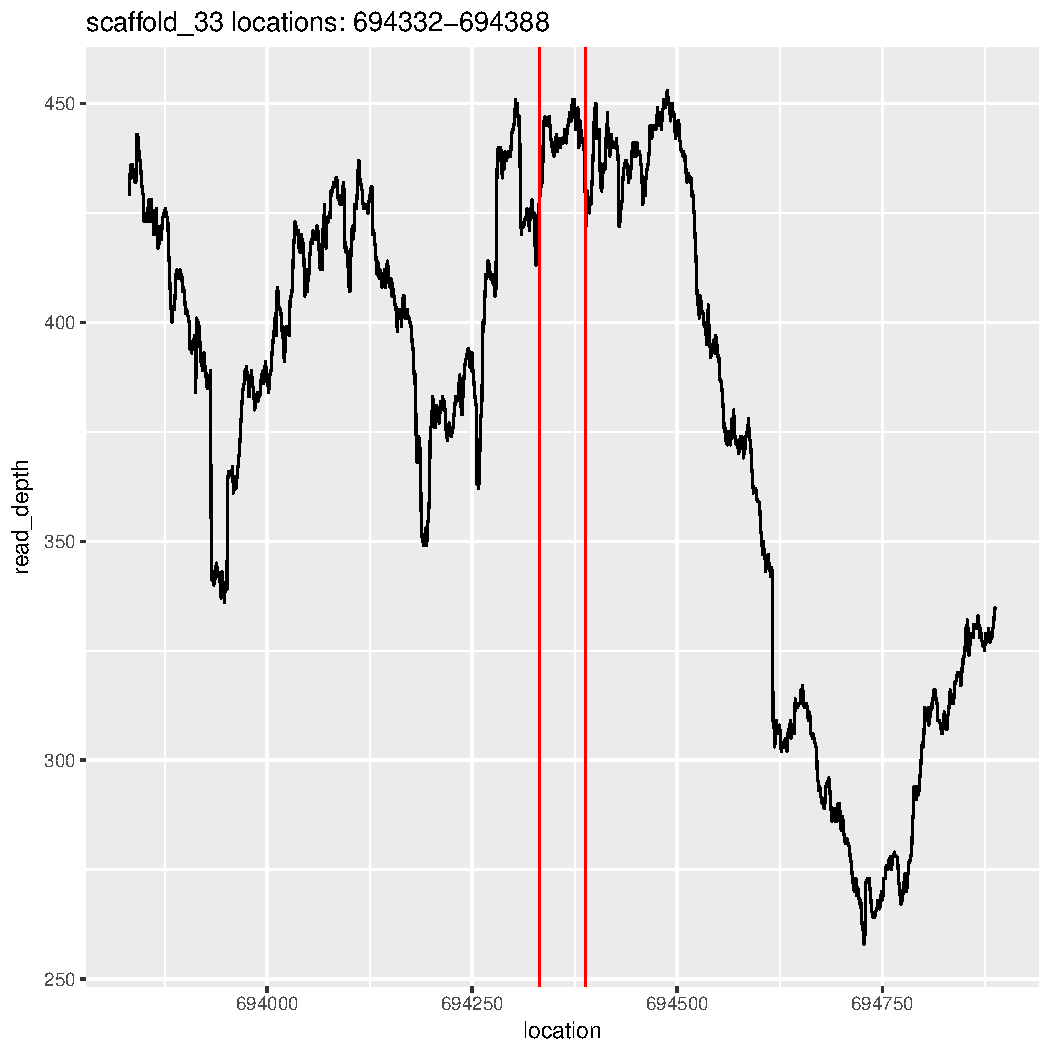
\includegraphics[angle=0,width=1.0\linewidth]{Figures/read_depth_snapsots/2100_Ar109_read_depth.pdf}}
		\resizebox{40mm}{40mm}{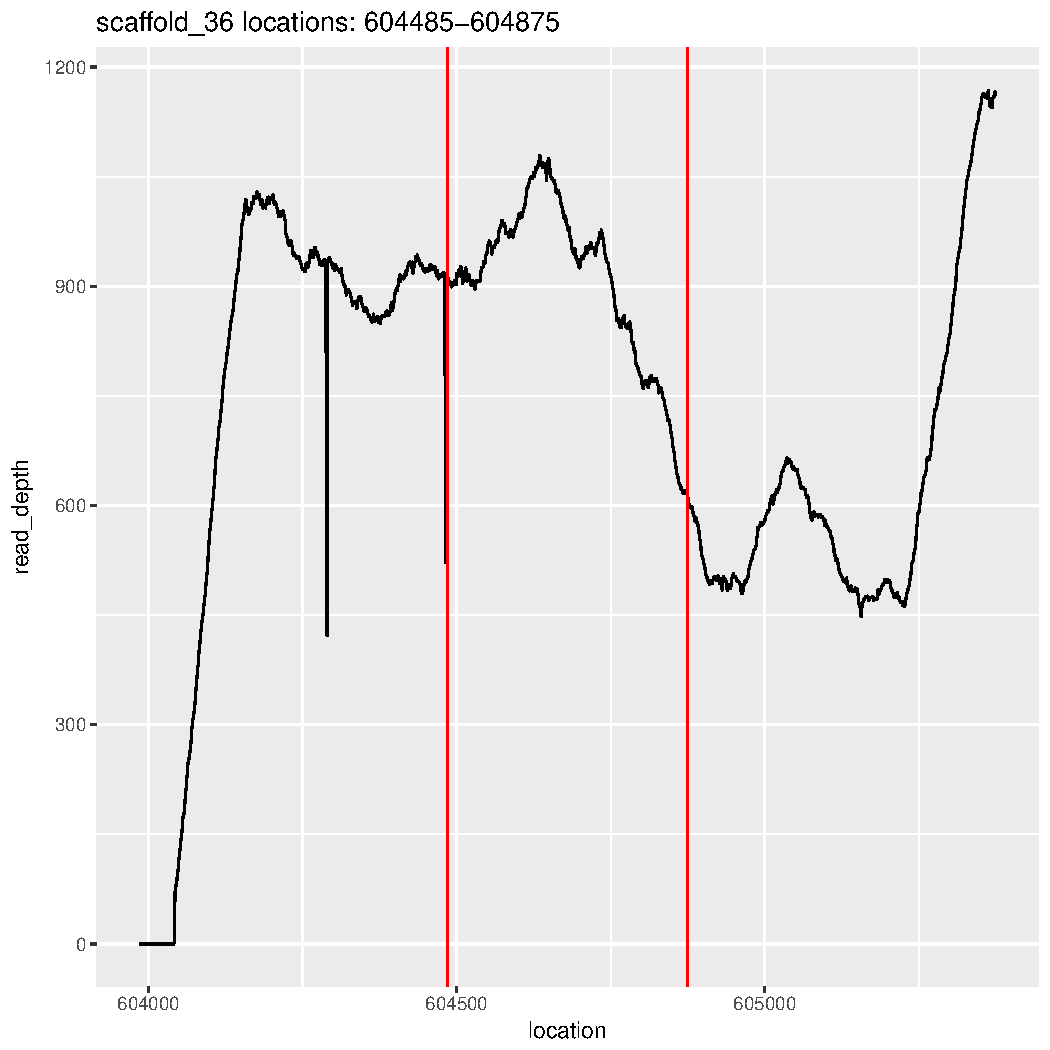
\includegraphics[angle=0,width=1.0\linewidth]{Figures/read_depth_snapsots/2200_Ar109_read_depth.pdf}}
		\resizebox{40mm}{40mm}{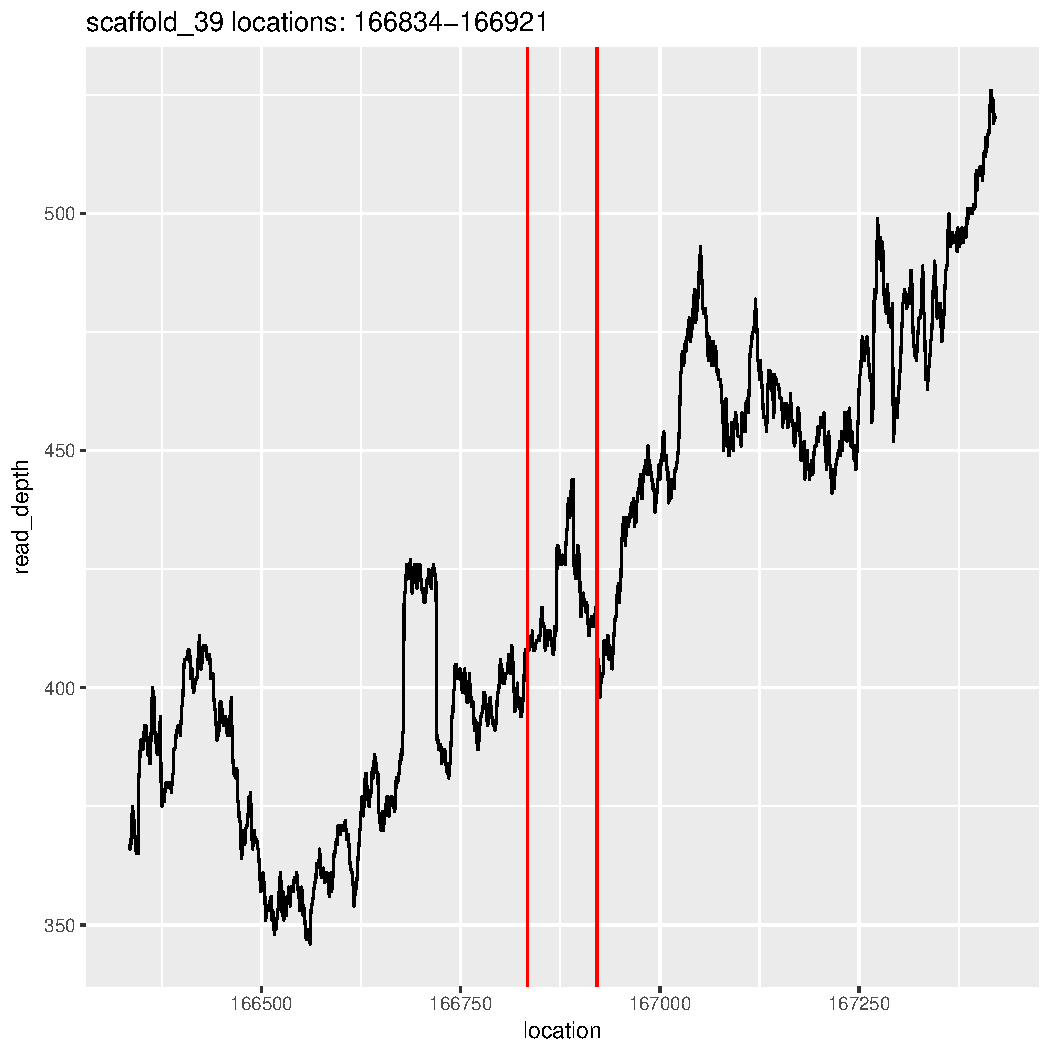
\includegraphics[angle=0,width=1.0\linewidth]{Figures/read_depth_snapsots/2300_Ar109_read_depth.pdf}}
		\resizebox{40mm}{40mm}{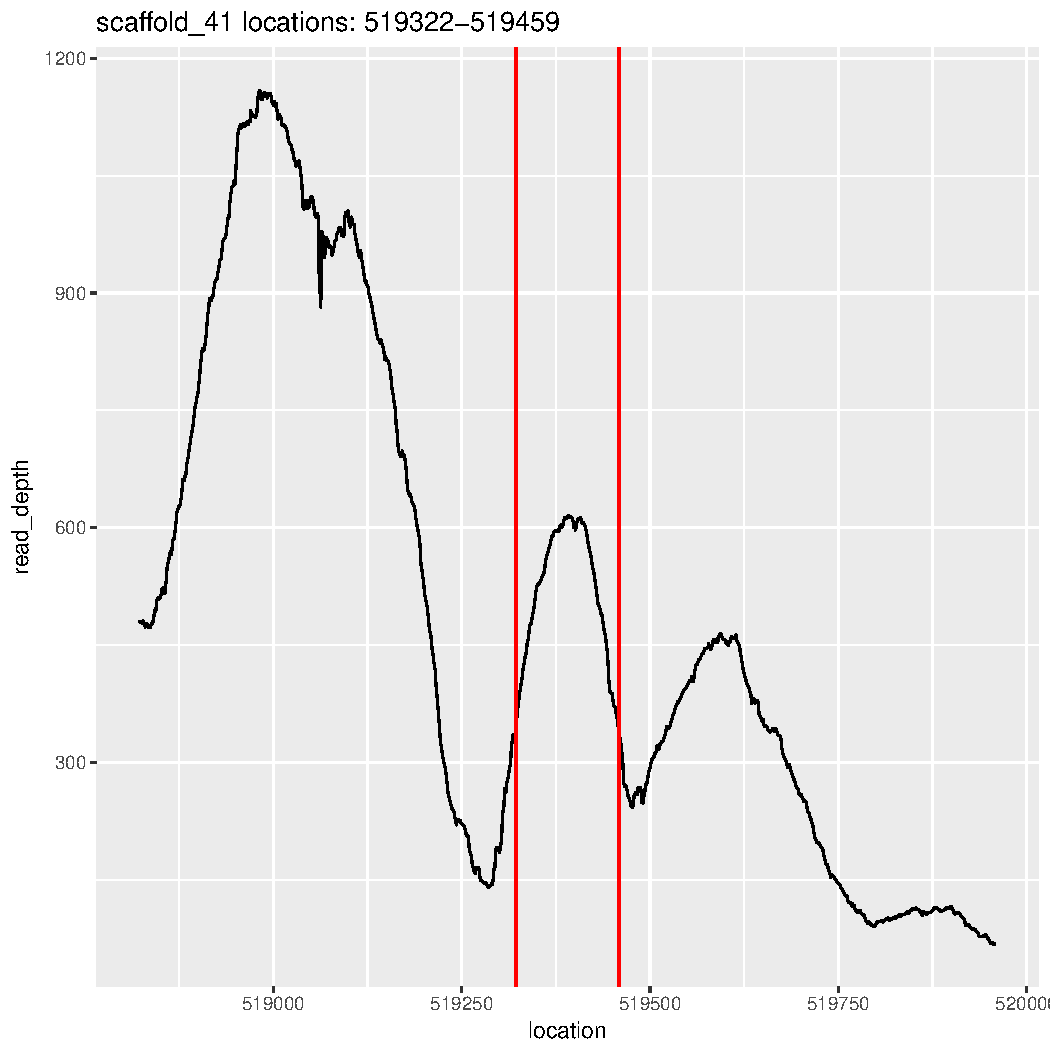
\includegraphics[angle=0,width=1.0\linewidth]{Figures/read_depth_snapsots/2400_Ar109_read_depth.pdf}}
		\resizebox{40mm}{40mm}{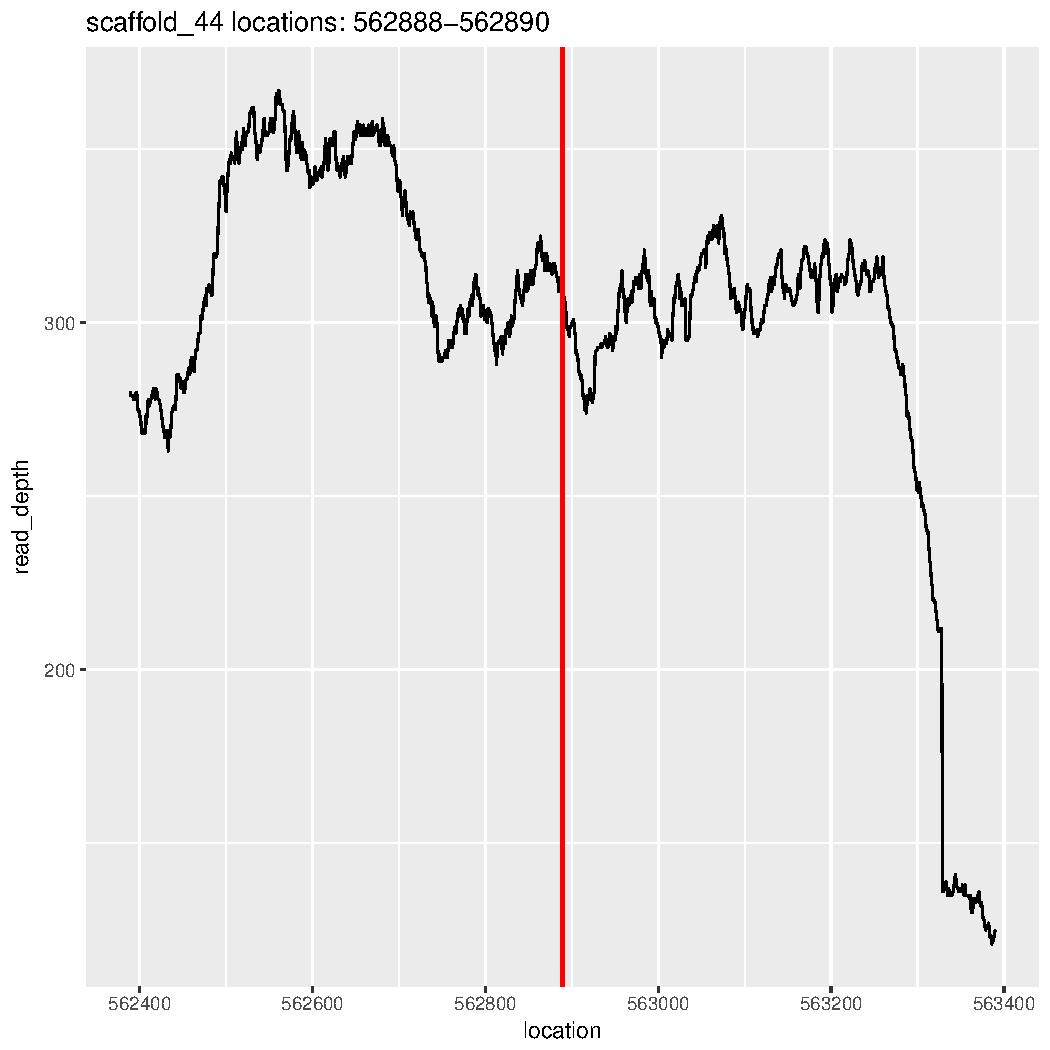
\includegraphics[angle=0,width=1.0\linewidth]{Figures/read_depth_snapsots/2500_Ar109_read_depth.pdf}}
		\resizebox{40mm}{40mm}{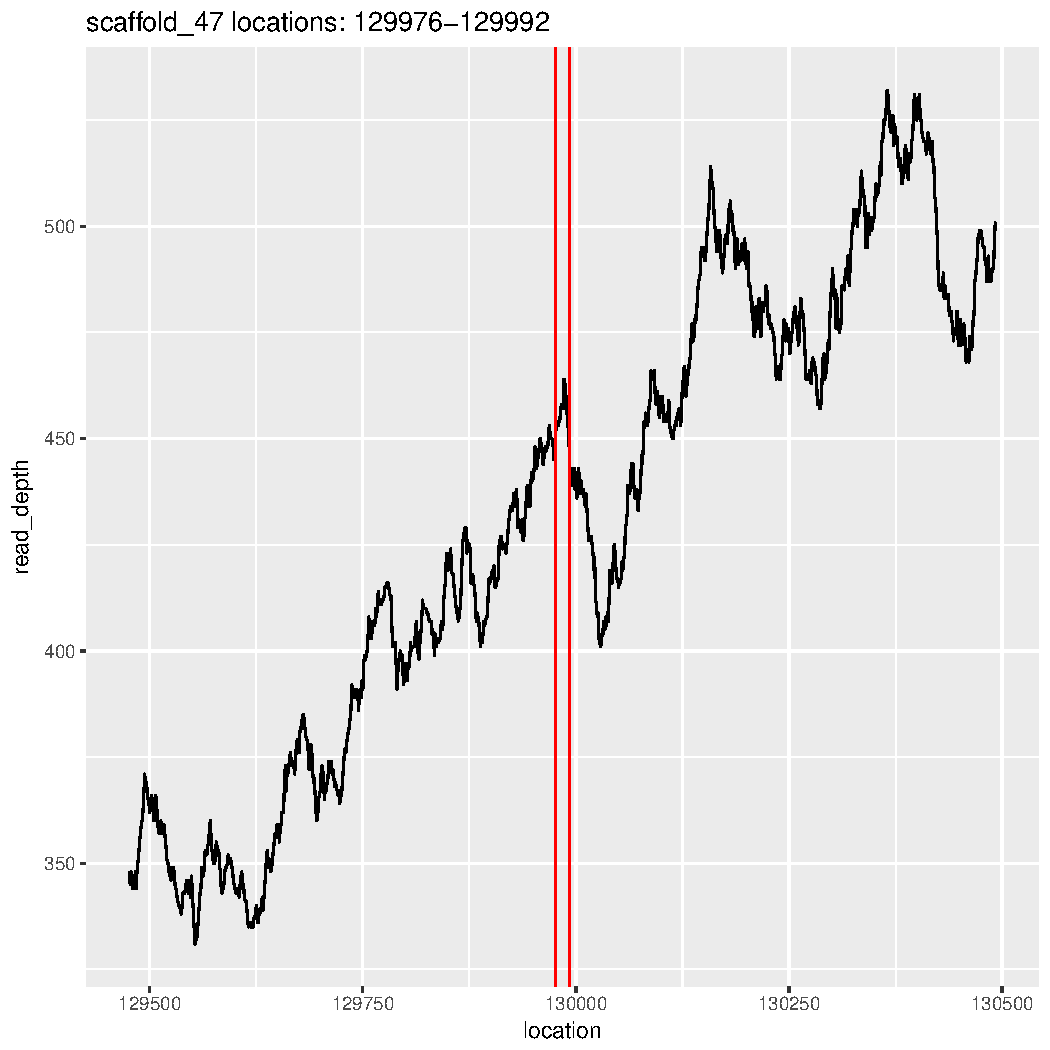
\includegraphics[angle=0,width=1.0\linewidth]{Figures/read_depth_snapsots/2600_Ar109_read_depth.pdf}}
		\resizebox{40mm}{40mm}{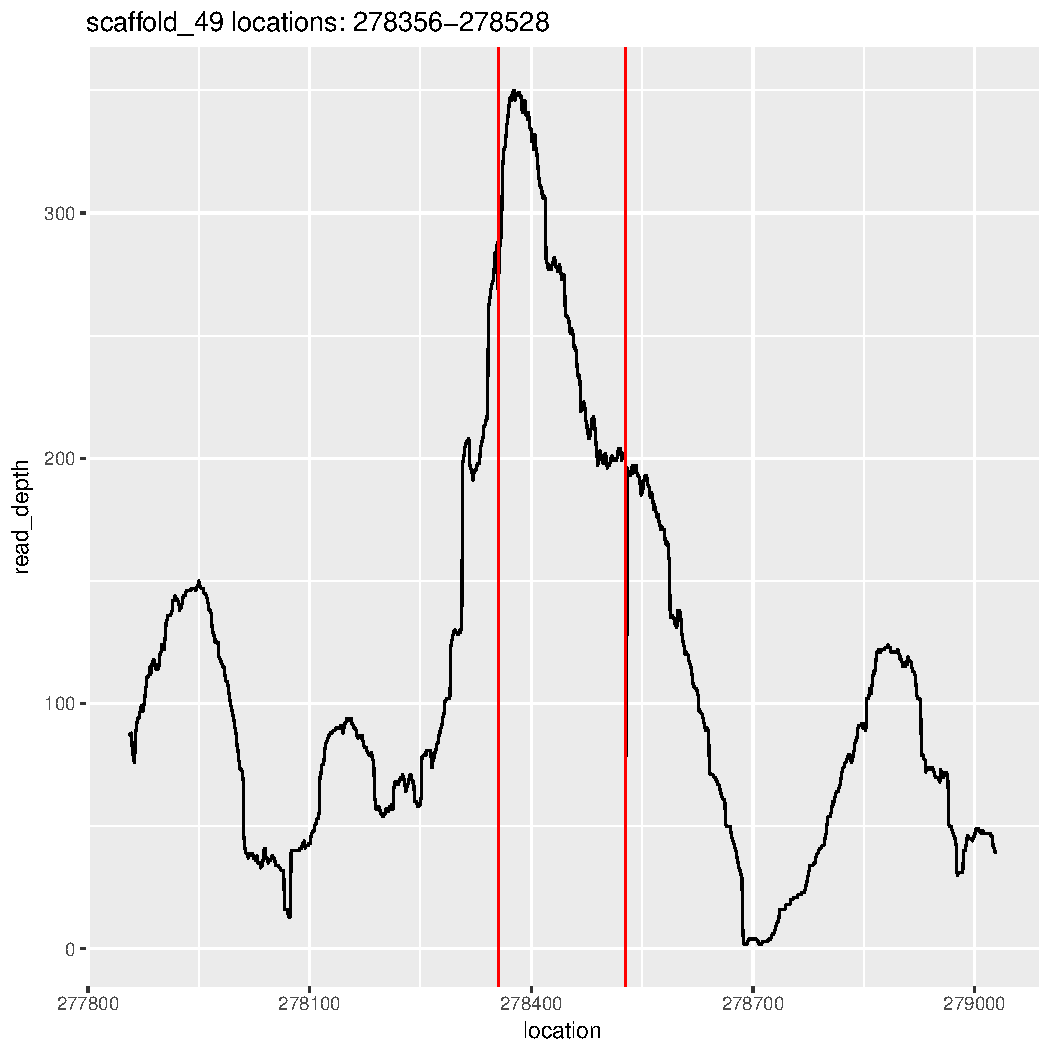
\includegraphics[angle=0,width=1.0\linewidth]{Figures/read_depth_snapsots/2700_Ar109_read_depth.pdf}}
		\resizebox{40mm}{40mm}{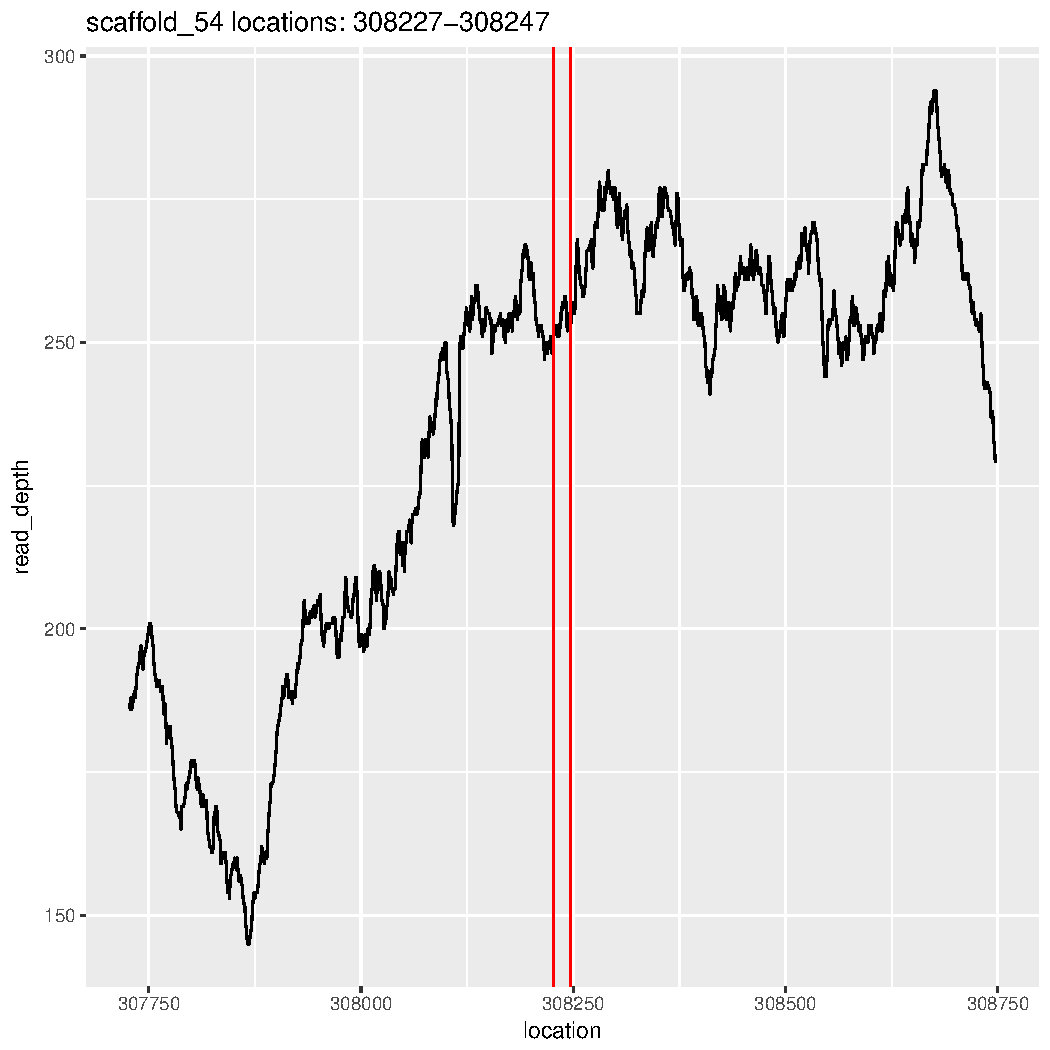
\includegraphics[angle=0,width=1.0\linewidth]{Figures/read_depth_snapsots/2800_Ar109_read_depth.pdf}}
		\resizebox{40mm}{40mm}{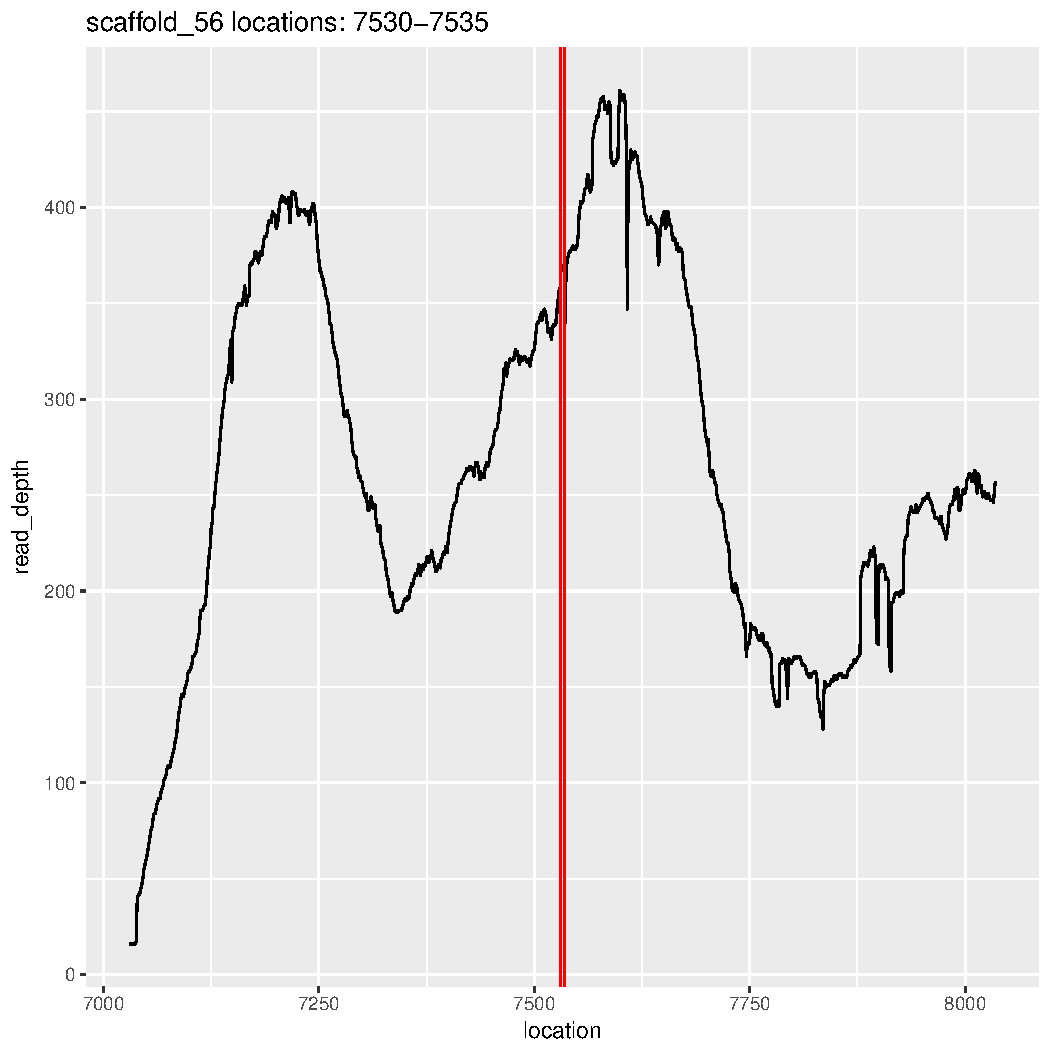
\includegraphics[angle=0,width=1.0\linewidth]{Figures/read_depth_snapsots/2900_Ar109_read_depth.pdf}}
		\resizebox{40mm}{40mm}{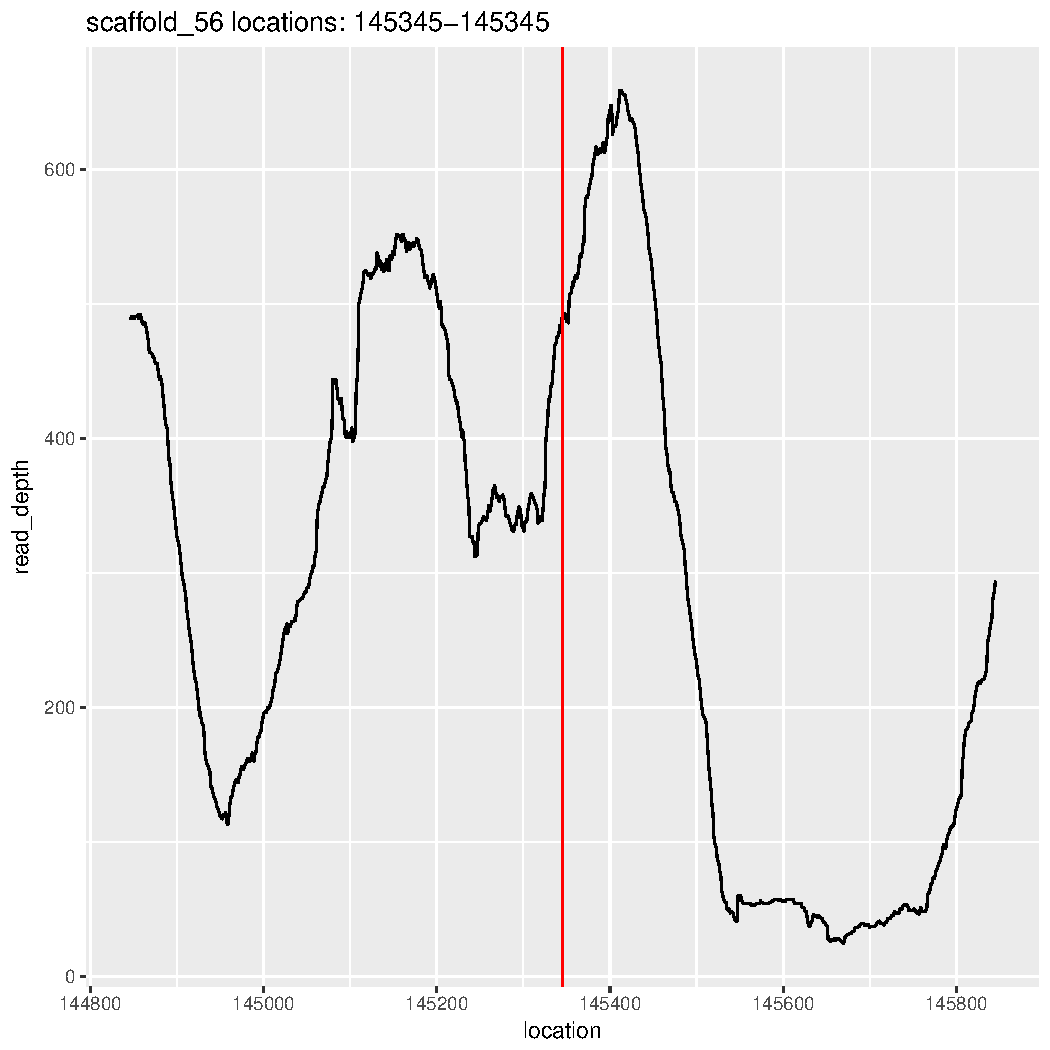
\includegraphics[angle=0,width=1.0\linewidth]{Figures/read_depth_snapsots/3000_Ar109_read_depth.pdf}}
		\resizebox{40mm}{40mm}{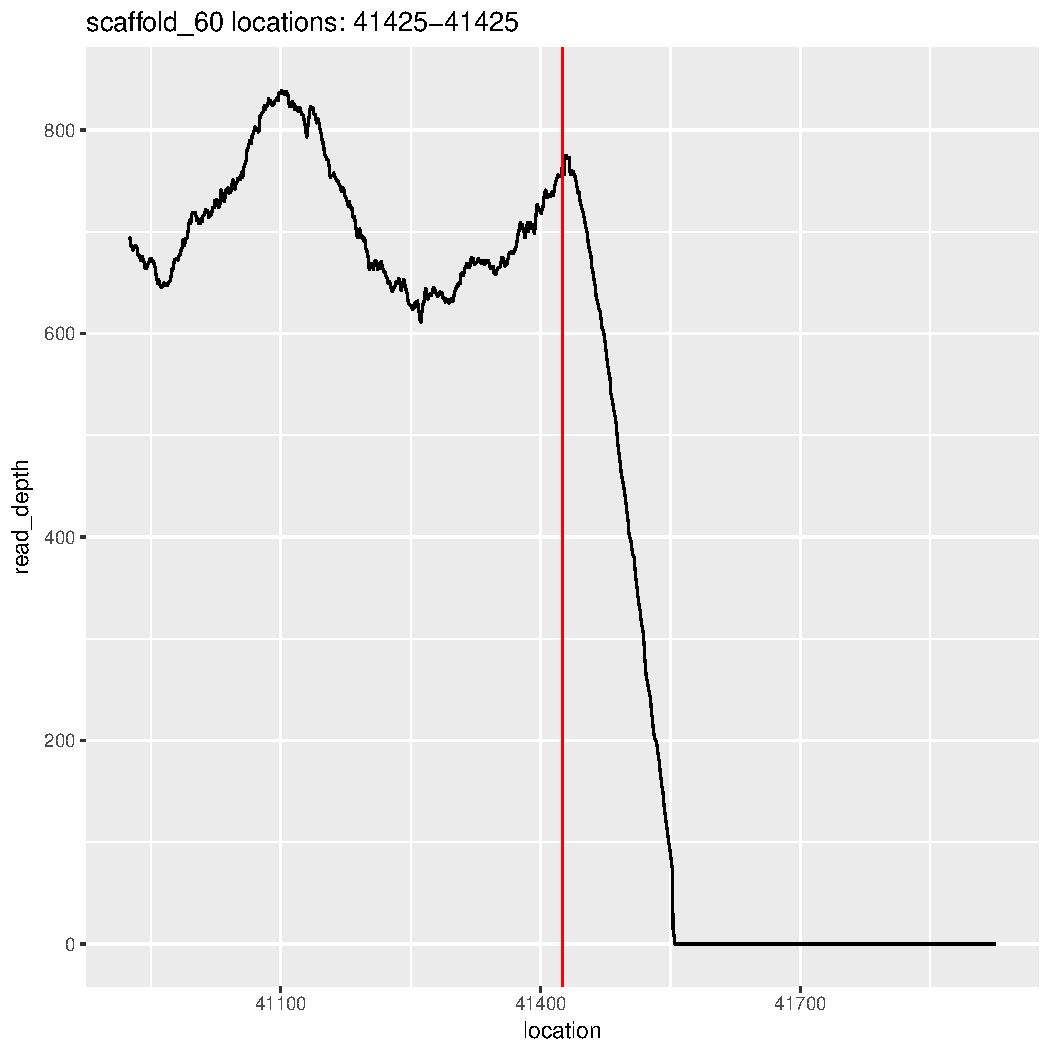
\includegraphics[angle=0,width=1.0\linewidth]{Figures/read_depth_snapsots/3100_Ar109_read_depth.pdf}}
		\resizebox{40mm}{40mm}{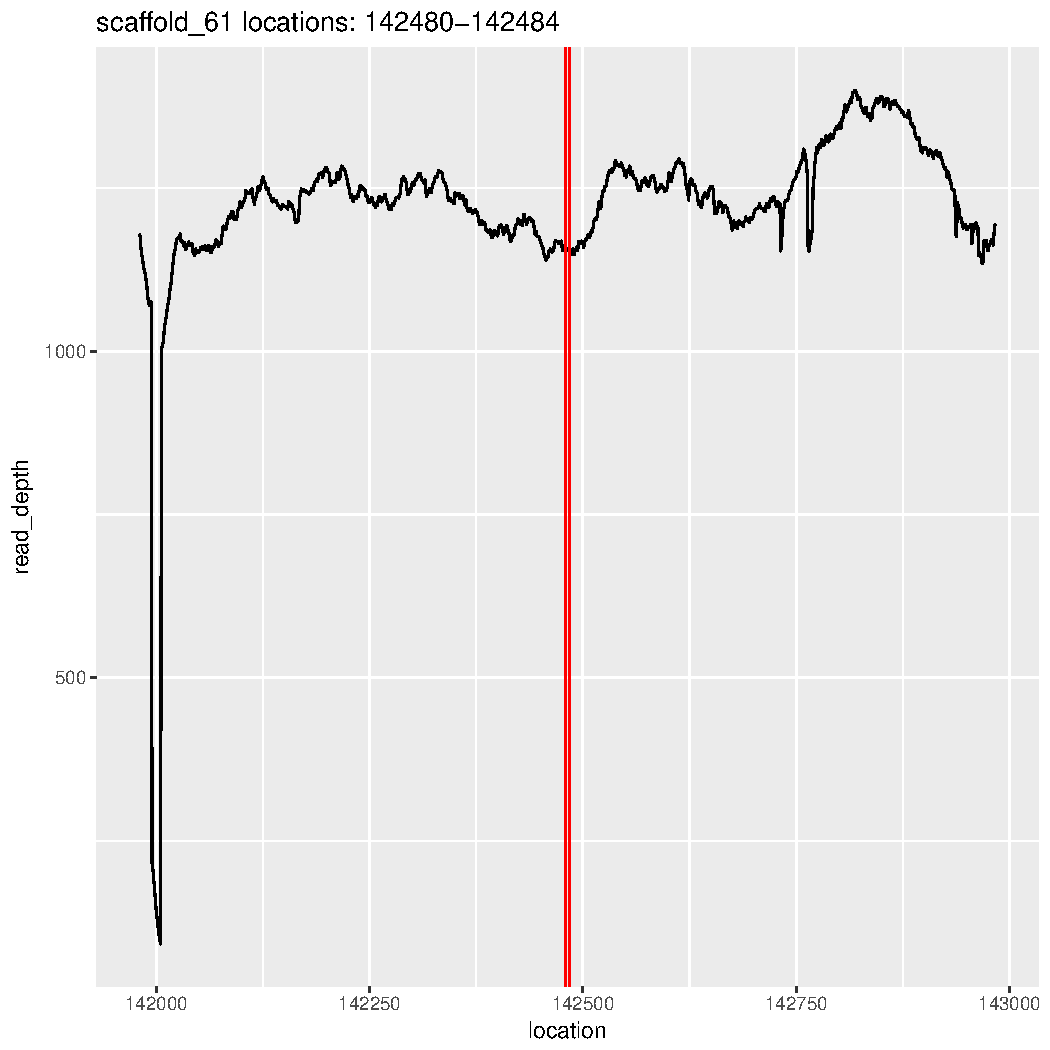
\includegraphics[angle=0,width=1.0\linewidth]{Figures/read_depth_snapsots/3200_Ar109_read_depth.pdf}}
		\resizebox{40mm}{40mm}{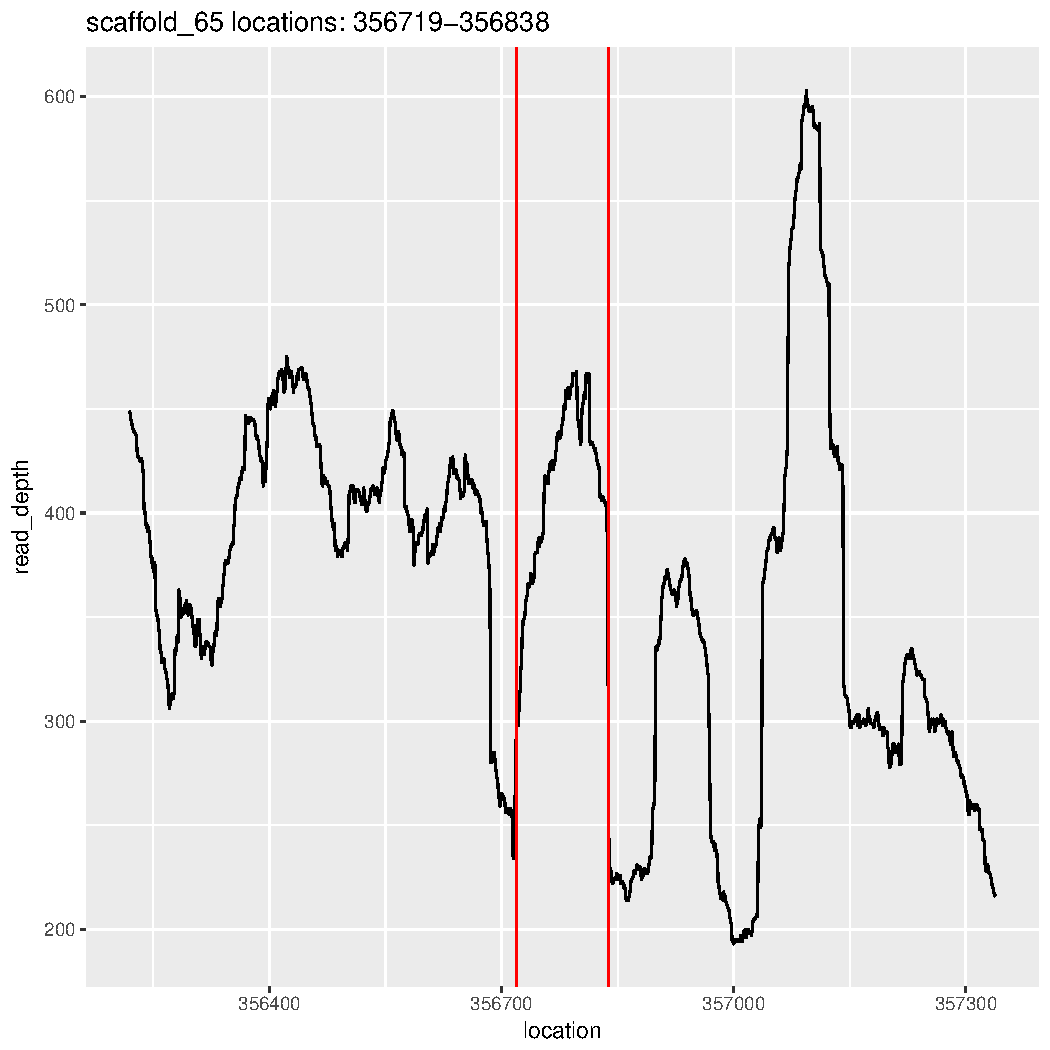
\includegraphics[angle=0,width=1.0\linewidth]{Figures/read_depth_snapsots/3300_Ar109_read_depth.pdf}}
		\resizebox{40mm}{40mm}{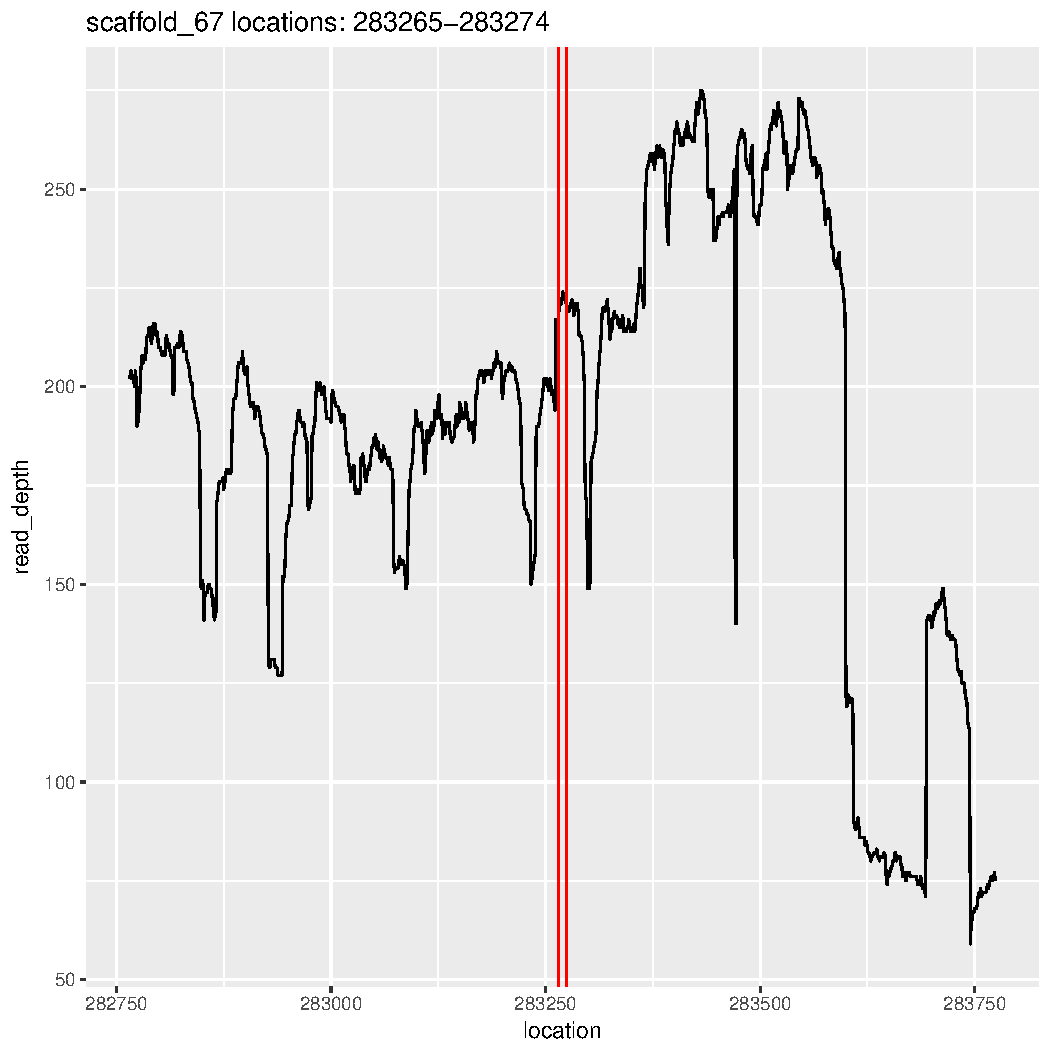
\includegraphics[angle=0,width=1.0\linewidth]{Figures/read_depth_snapsots/3400_Ar109_read_depth.pdf}}
		\resizebox{40mm}{40mm}{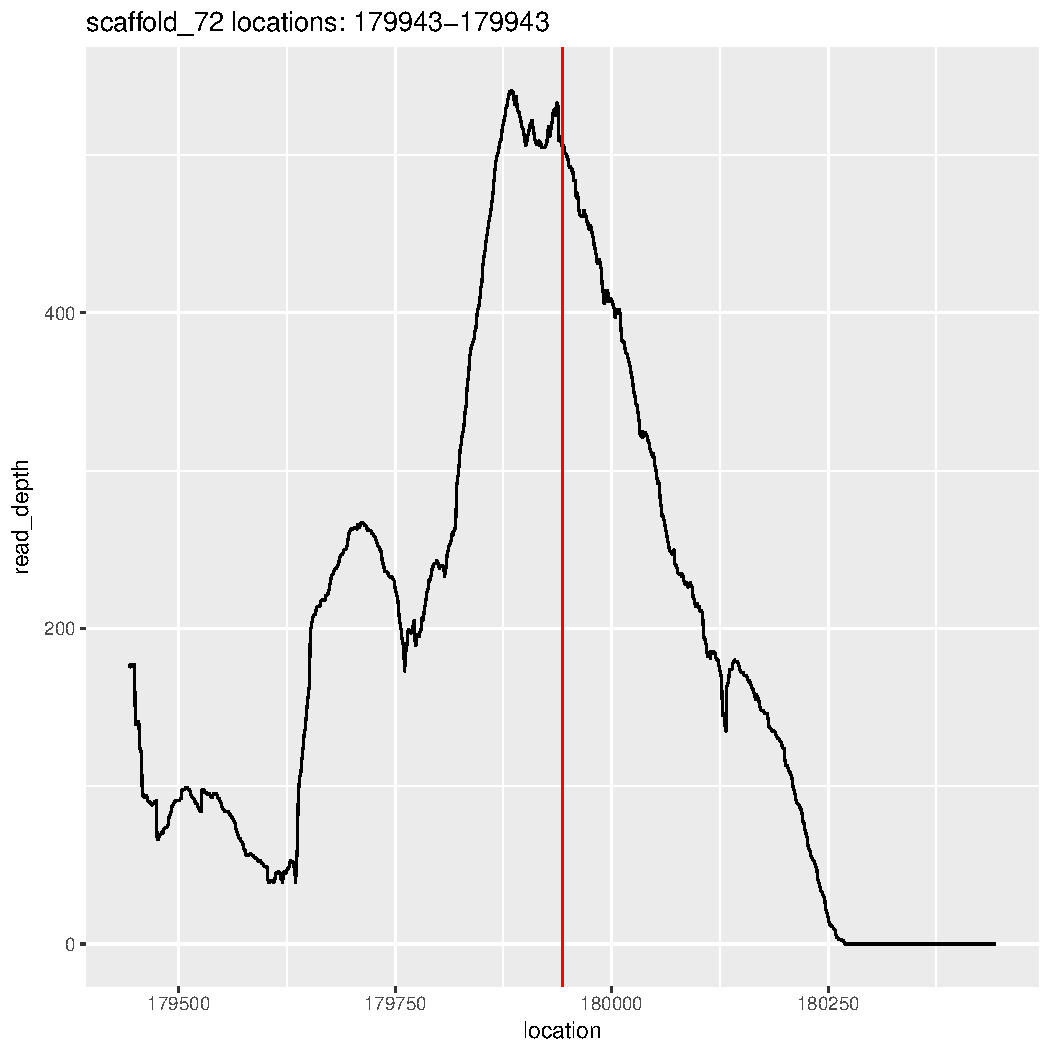
\includegraphics[angle=0,width=1.0\linewidth]{Figures/read_depth_snapsots/3500_Ar109_read_depth.pdf}}
		\resizebox{40mm}{40mm}{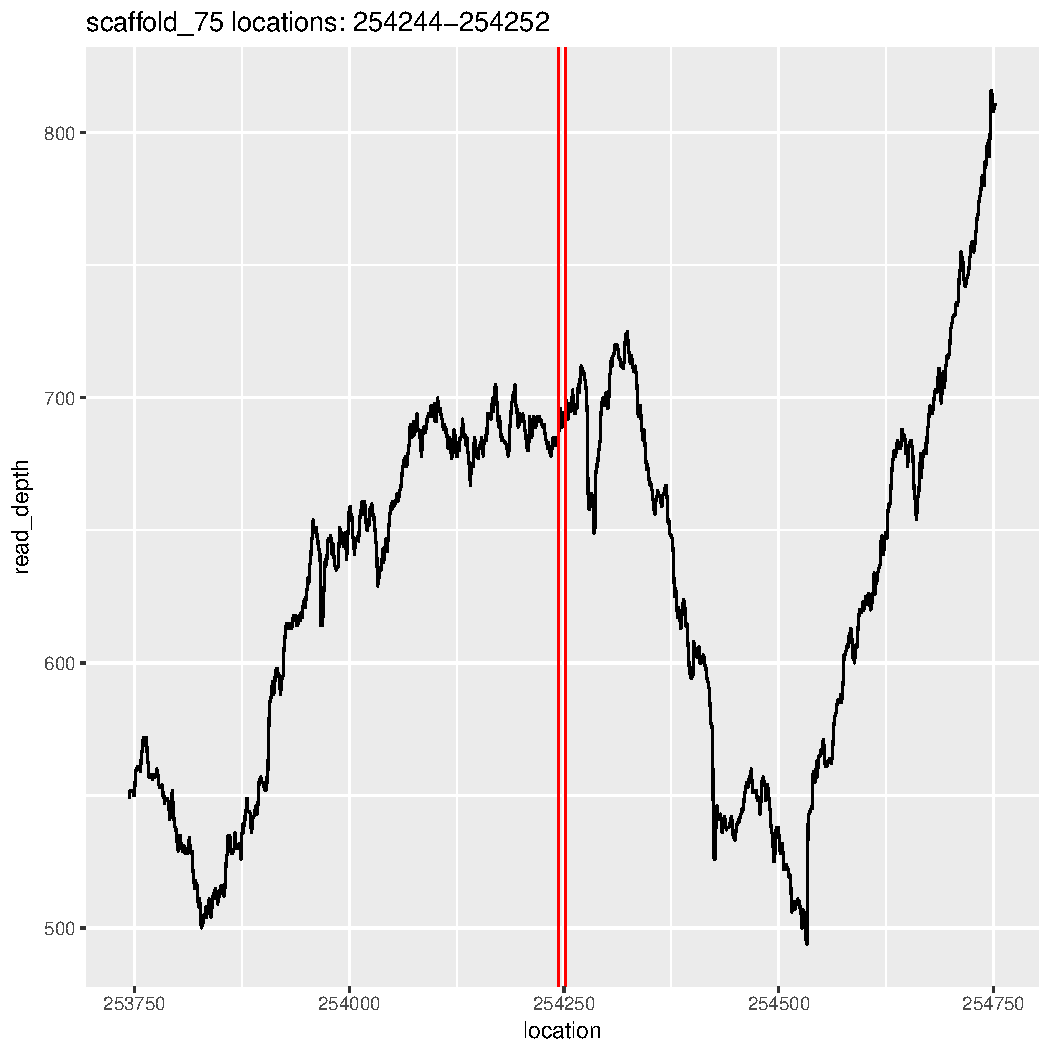
\includegraphics[angle=0,width=1.0\linewidth]{Figures/read_depth_snapsots/3600_Ar109_read_depth.pdf}}
		\resizebox{40mm}{40mm}{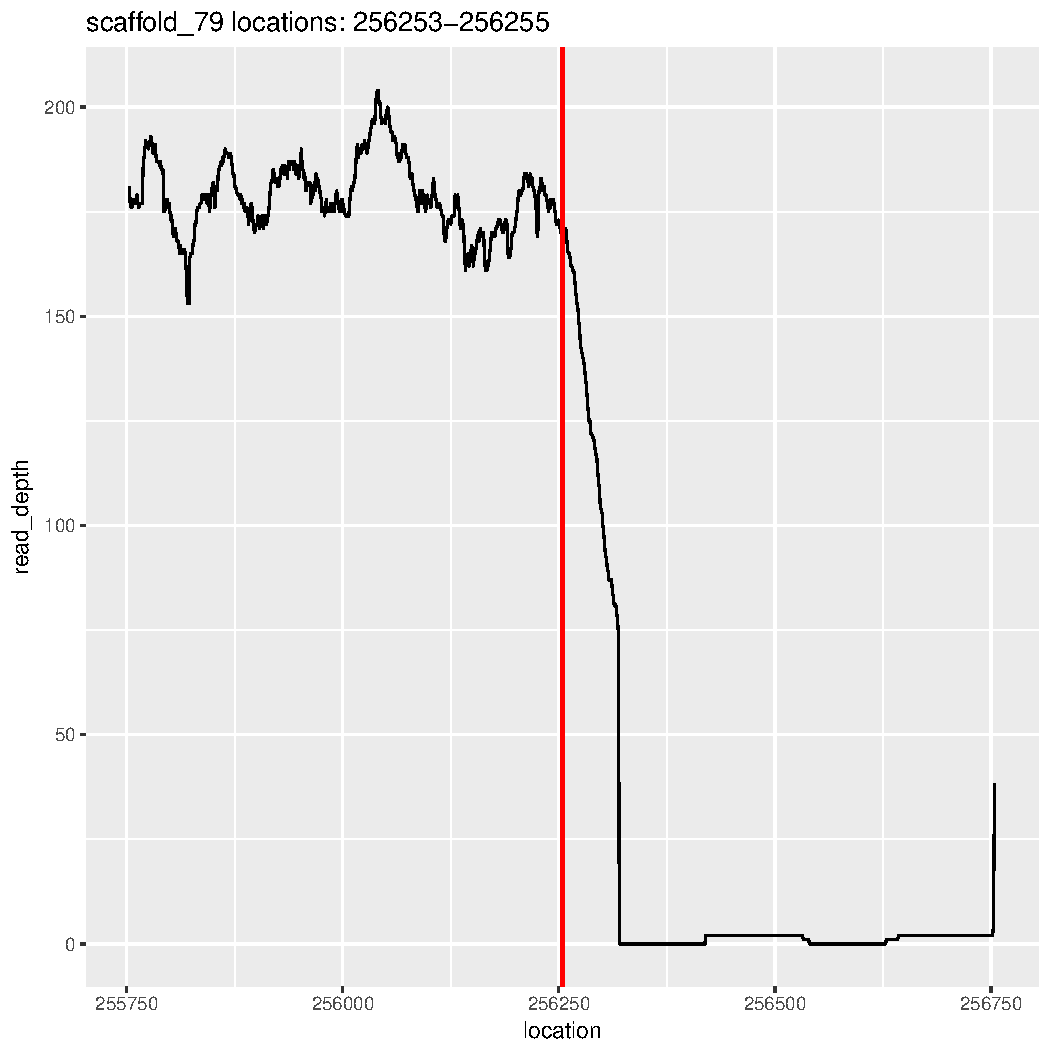
\includegraphics[angle=0,width=1.0\linewidth]{Figures/read_depth_snapsots/3700_Ar109_read_depth.pdf}}
		\resizebox{40mm}{40mm}{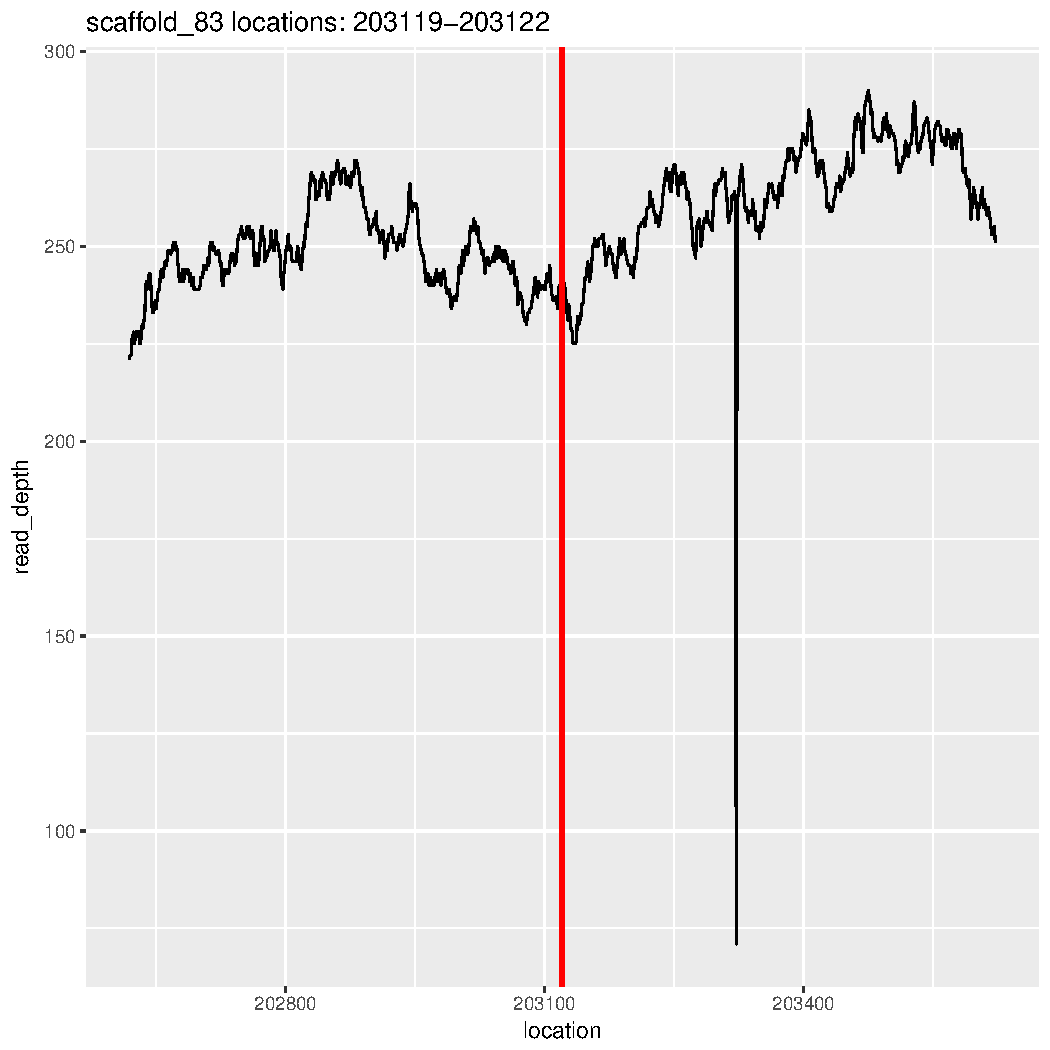
\includegraphics[angle=0,width=1.0\linewidth]{Figures/read_depth_snapsots/3800_Ar109_read_depth.pdf}}
		\resizebox{40mm}{40mm}{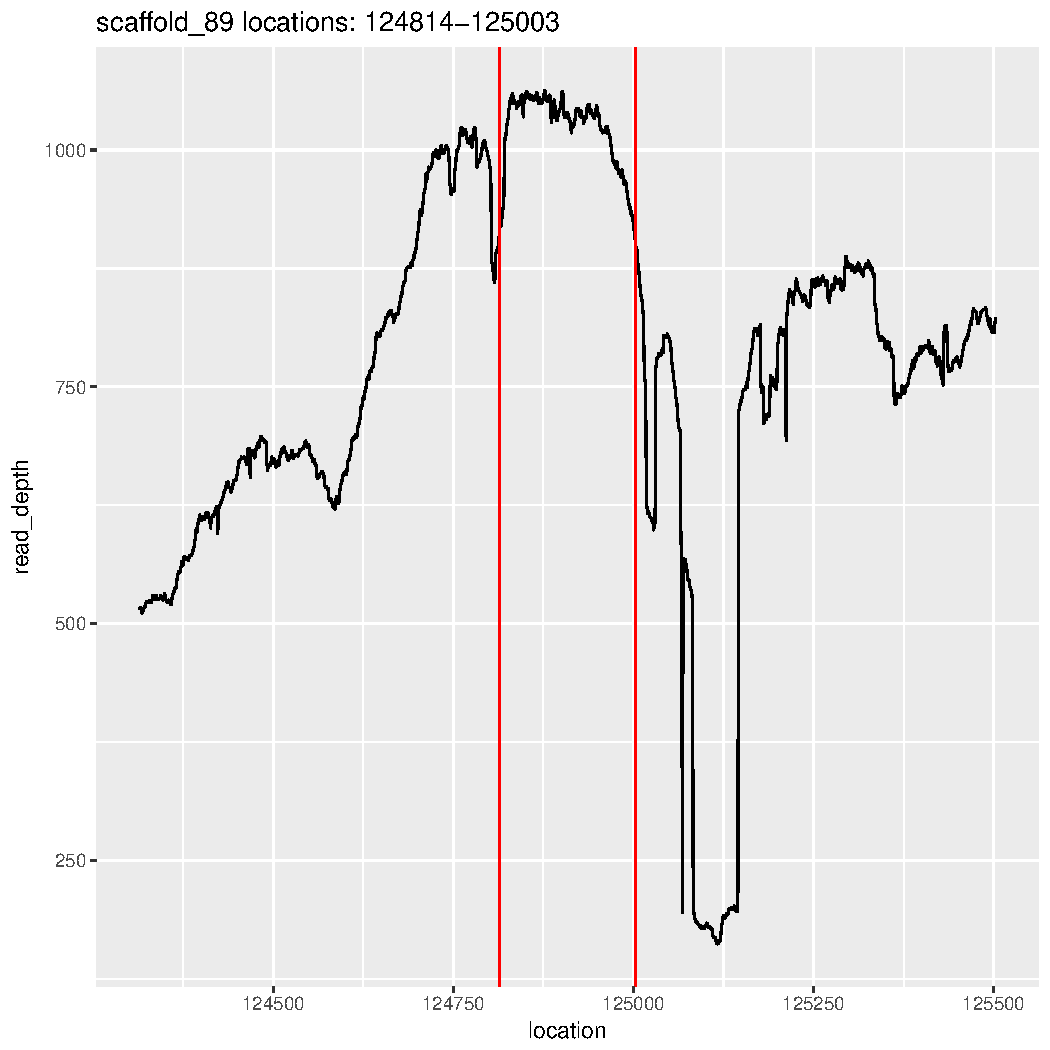
\includegraphics[angle=0,width=1.0\linewidth]{Figures/read_depth_snapsots/3900_Ar109_read_depth.pdf}}
		\begin{singlespace}
			\vspace{-0.5cm}
			\caption[Average Read Depth Snapshots]{Average Read Depth Snapshots. Graphs are of locations 1, and every 100 starting at 2000 until 3900.}\label{avg_rd_snpsht_2}
		\end{singlespace}
	\end{centering}
\end{figure}

\newpage
Additionally I have created a graph showing the total read depth across each scaffold. Example below.

\begin{figure}[H]
	\begin{centering}
		\resizebox{150mm}{60mm}{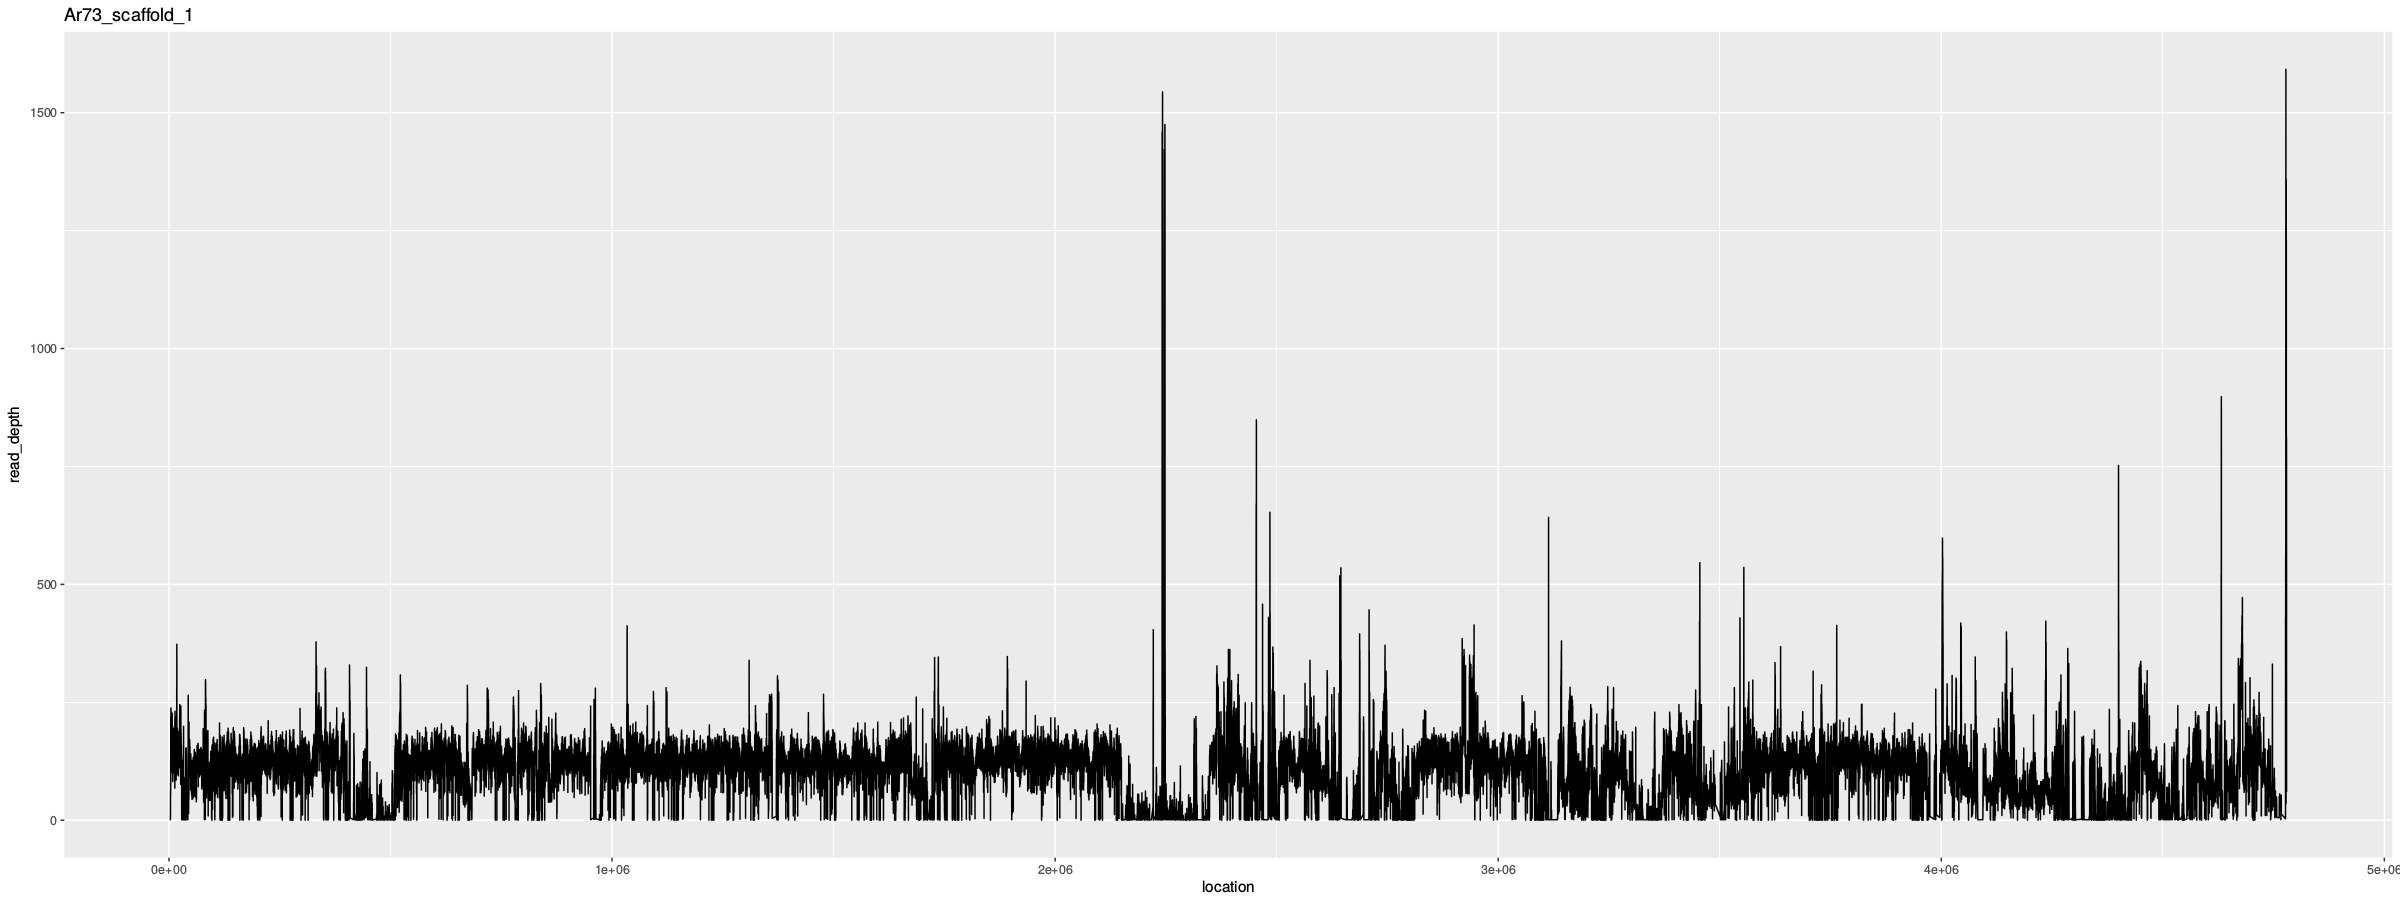
\includegraphics[angle=0,width=1.0\linewidth]{Figures/Scaffold_read_depth_graphs/Ar73_scaffold_1_read_depth.pdf}}
		\resizebox{150mm}{60mm}{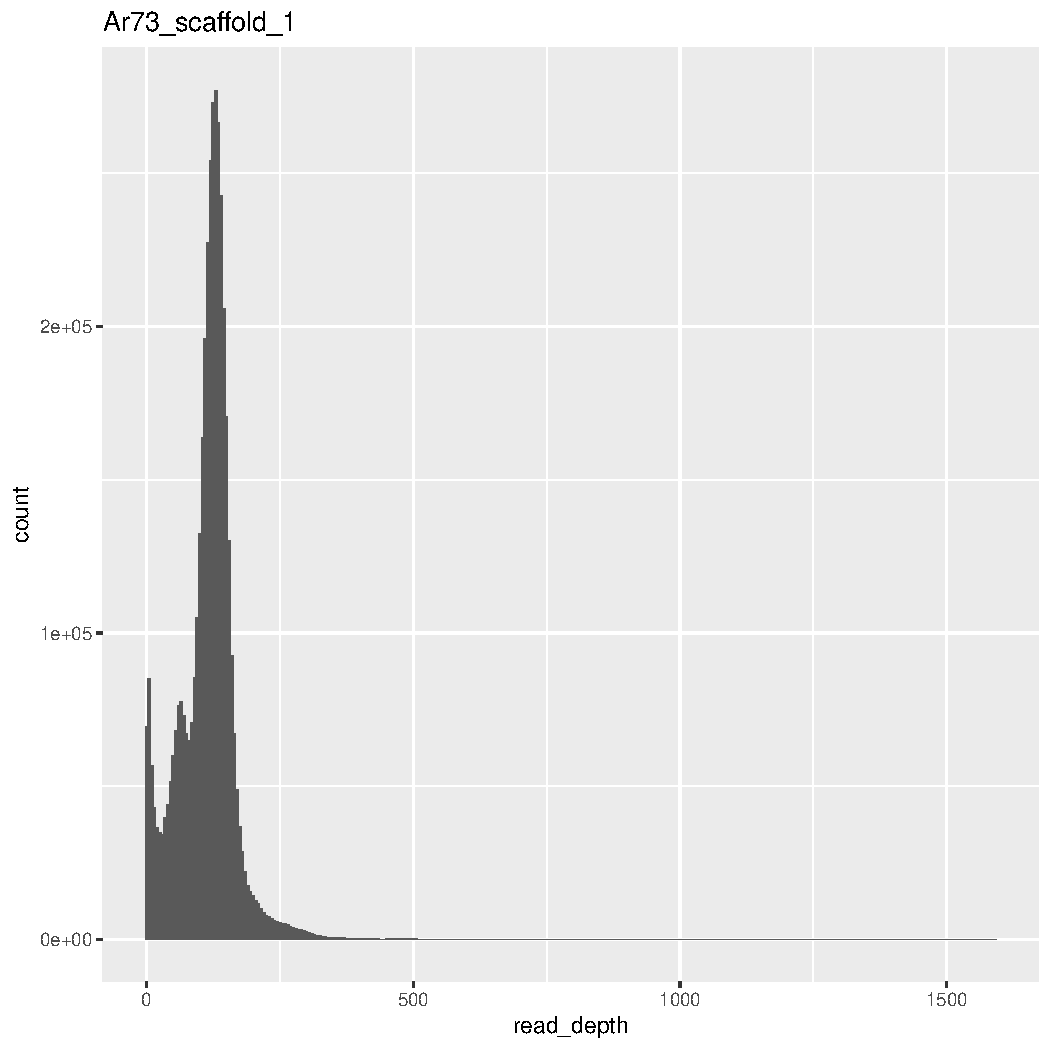
\includegraphics[angle=0,width=1.0\linewidth]{Figures/Scaffold_read_depth_graphs/Ar73_scaffold_1_read_depth_histogram.pdf}}
				\begin{singlespace}
			\vspace{-0.5cm}
			\caption[Global Scaffold Read Depth Example]{Global Scaffold Read Depth Example for Ar73, scaffold 1.}\label{global_scaff_rd}
		\end{singlespace}
	\end{centering}
\end{figure}

\end{document}
